% design.tex
\chapter{Design}
In this section of my NEA I will be including details on the detailed design of my Journal app. 


\section{Introduction}
The objective of my journal app is to provide users with an easily accessible and navigated app for digital journaling. To accomplish this, I will choose the Django REST framework for my backend server functionality and React, a powerful JavaScript library, for my frontend. In this section of my report I will be justifying why I have made these choices and detailing the specific designs for full stack application tailored to these frameworks

\section{Frontend}
Frontend primarily refers to the interface which the user interacts. The most common form of frontend is a webpage, which encompasses the layout and design elements of the website. Initially, webpages are created using HTML, CSS, and JavaScript. However, as time progresses, developers have devised ways to generate them. Using Python, for example, frameworks like Django and Flask allow developers to build HTML, CSS, and Javascript pages interactively and dynamically. In the case of Django and Flask, developers can use templating engines like Jinja2 to generate dynamic HTML pages by integrating Python code into the HTML layout, as well as being able to avoid boilerplate code by building templates for the layout of the appearance of the page and then being able to make changes to different pages while maintaining consistency across the website. This approach saves time since it lets me focus on the features instead of writing boilerplate code.

Behind the scenes, frontend is not only the UI, as it also includes the logic and functionality that drives the user experience. This includes handling user interactions, making API calls, data manipulation, and updating the UI based on user input.

Javascript frameworks are the most popular amongst web developers since there exist powerful libraries like React and Angular maintained by giant tech companies, and javascript is simply more widely adopted and used in the web development world. Similarly, I have heard good things about a library called Svelt, which offers a lightweight approach to building user interfaces. What I mean by that is it uses fewer codes, is truly reactive, and has no virtual DOM

Initially, I used Django to generate my frontend pages using its built-in templating engine dynamically. However, I want to create a more modular approach and, therefore, truly isolate my backend and frontend. The benefit of doing so is that I could connect a completely different front-end interface to the same backend functionality with ease via API communication. In my application, I will try my best to maintain the Single Responsibility design principle throughout my application development process.\\
To achieve achieve this modular approach, I decided to use a separate frontend to my Django backend, specifically React.js. React is the most popular and in-demand ecosystem developed by Facebook for building responsive user interfaces, Facebook developed React.js and later React native for building "truly native" mobile apps using JavaScript. React.js is the javascript library I chose for my web creation, and I believe that it would be a valuable learning experience to take on my first Javascript library to build my app.

\section{Backend}
Backend refers to the server side of a web application, where the logic behind the application is. It is responsible for processing requests, interacting with databases, and algorithmically generating responses to be sent back to the client and other background processes. There are frameworks available for different programming languages that can be used for backend development.

I have considered Python, C\# and Javascript frameworks for my project as I am proficient in Python, C\# (having dabbled with those in my own time and studied those languages for GCSE and A-Levels, respectively), and Javascript is a language I have always wanted to explore further since it is the most popular language; hence, there's wide support for it in terms of libraries and frameworks. Specifically, I have considered Django, FastAPI, Flask, Next.js, and ASP.NET Core frameworks.

\subsection{ASP.NET:}
ASP.NET is a powerful framework developed by Microsoft for building web apps and services using the .NET framework and C\#. It is capable and scalable, making it suitable for large-scale applications. Personally, however. I did not end up choosing ASP.NET due to my hardware constraint. I am running a MacOS unix system on the apple silicone architecture, which I could technically do .Net development using. However, from my experience in the past, it is a pain. In addition, ASP.NET was primarily suited for the Windows ecosystem (although they are trying to make it more platform-independent), meaning it is not optimal for me personally, and there are other better ways to create a university platform-independent backend.

\subsection{Next.js and Express.js:}
Two of the most demanding and powerful frameworks are these two are used to build the backend using Node.js. Next.js goes hand-in-hand with React since it provides server-side rendering. This is a thin client approach, where the initial HTML is generated on the server and then sent to the client. This approach ensures the smoothness of the user experience \cite{gillis_2020_fat}. Express.js is, on the other hand, a lightweight and flexible framework for building RESTful APIs and the like. It might be nice, but I am more comfortable with Python, so I decided that it's a good idea to only use Javascript for my Frontend development and Python for my Backend.

\subsection{Flask and FastAPI:}
Flask is a lightweight web framework for Python used to build APIs. I had previously dabbled with the framework and found it barebone and flexible. FastAPI is a much more modern alternative to Flask. It provides similar simplicity and flexibility but with the added benefit of high performance due to its asynchronous capabilities. I was really tempted to use FastAPI for my project, however, I had been learning a lot of Django and decided to go with it instead.

\subsection{Django}
Django is the most feature-rich mainstream backend web development framework in Python. It provides all the necessary tools I need, including URL routing, Database Object-Relational mapping, as well as overall security features preventing basic forms of attacks such as CSRF. This allows me to robustly build my application, focusing on functionalities that matter rather than reinventing the wheels. Django also allows me to have fine-tuned control over functionalities if I want to redesign, replace, or extend any parts. Even though Django might not be as performant as some other frameworks, such as FastAPI, it offers a well-established and stable platform for web development suitable for my Journal app.

\section{Hierarchy Charts}
Hierarchy charts are visual representations of a large problem being broken down into smaller components or sub-problems. They are charts in the form of an upside-down tree structure. Ideally, the problem should be broken down until each module is no longer than a page of code. In the charts I have created, I had to separate my application for two different charts. One for my Frontend and one for my Backend because the project is quite large. In the diagram, I have broken down my problems to a reasonably small size yet not too specific such that it becomes too difficult to maintain.

\subsection{Django Server Design:}
In this hierarchy chart, I have decomposed the design of my entire Django backend API into many smaller problems I will solve in my implementation. I will not be describing each individual problem in detail here. Still, the hierarchy chart provides a clear overview of how the different components and functionalities of the backend system are organised. See Figure \ref{fig:backendHD} for the chart.

\subsection{React Frontend}
In the hierarchy chart for the JavaScript frontend, I have broken down the design of my user interface and client-side functionalities into smaller components.

These components include user authentication, data retrieval from the backend API, the UI and more. In this chart, it's hard to show how the functions communicate at an inter-component level. However, on top of what's designed in the hierarchy chart, data is passed through props and the things under my state management box shown in the diagram would be accessible throughout my application by different components through the use of React Context and Context Provider. See Figure \ref{fig:frontendHD} for the chart.

\begin{landscape}
\begin{figure}
    \centering
    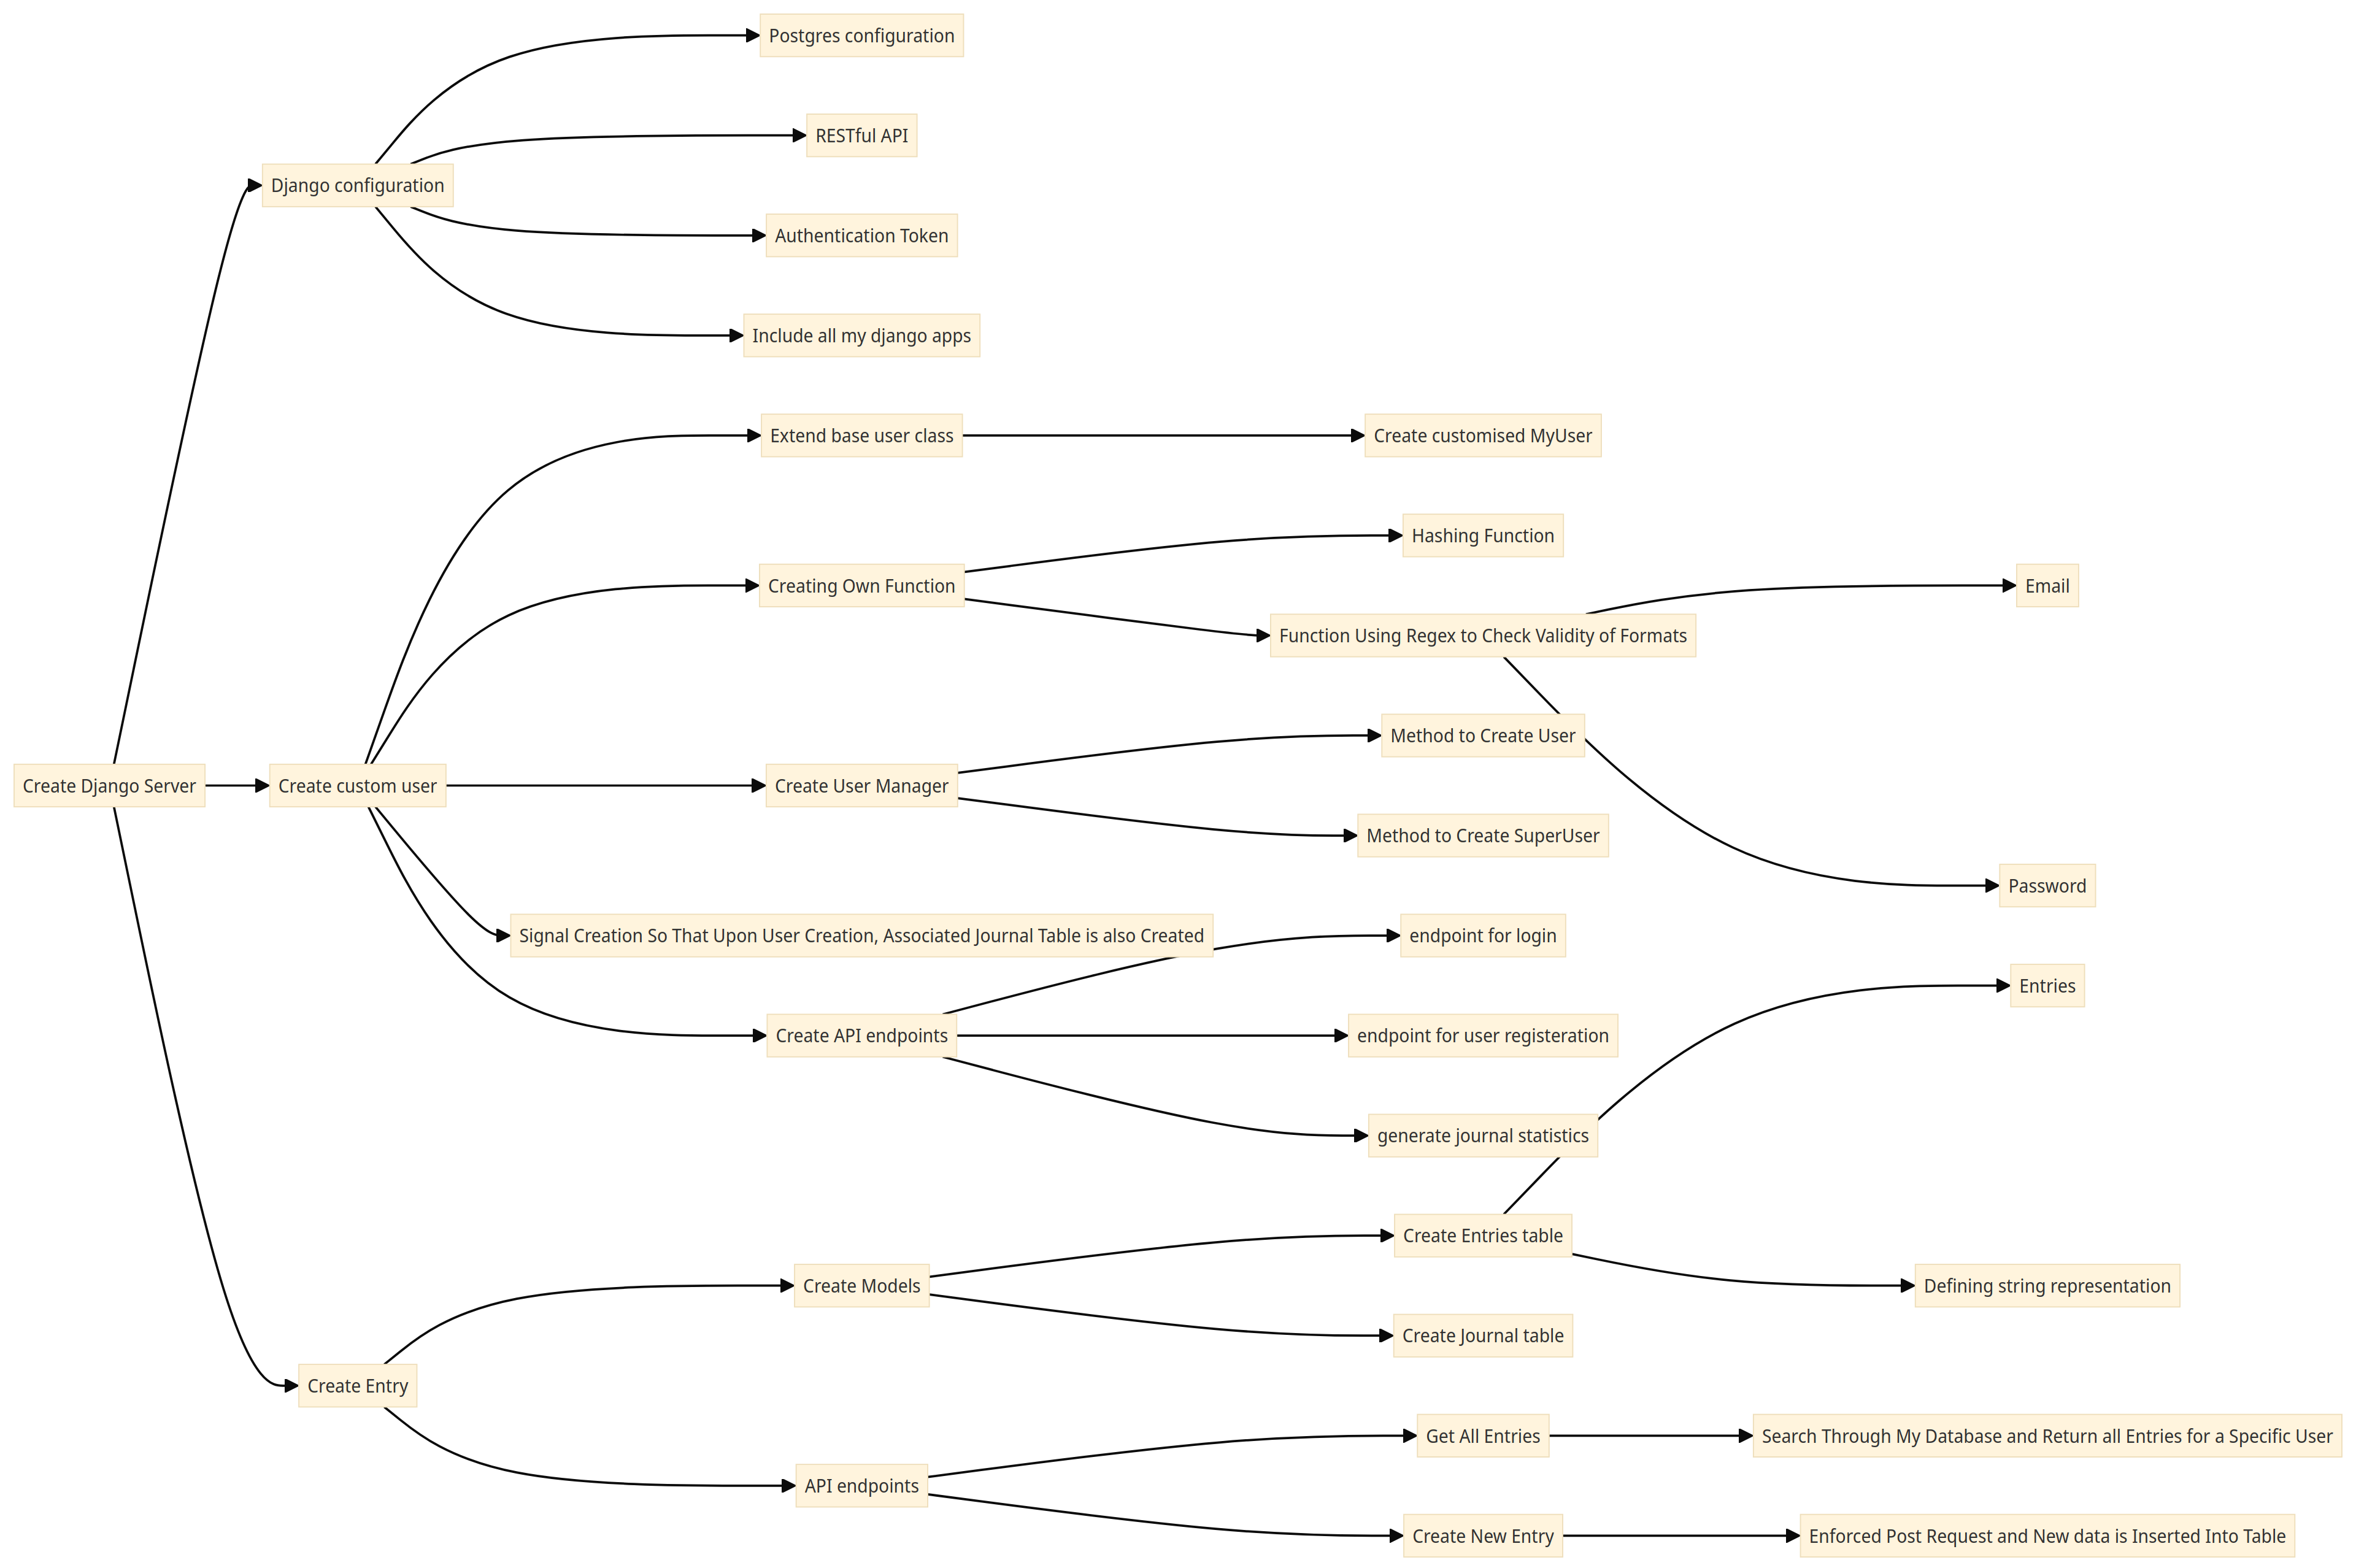
\includegraphics[
    width=1\linewidth,
    ]{Assets/Hierarchy_Backend.png}
    \caption{Backend Hierarchy Diagram}
    \label{fig:backendHD}
\end{figure}
\end{landscape}



\begin{landscape}
    \begin{figure}
        \centering
        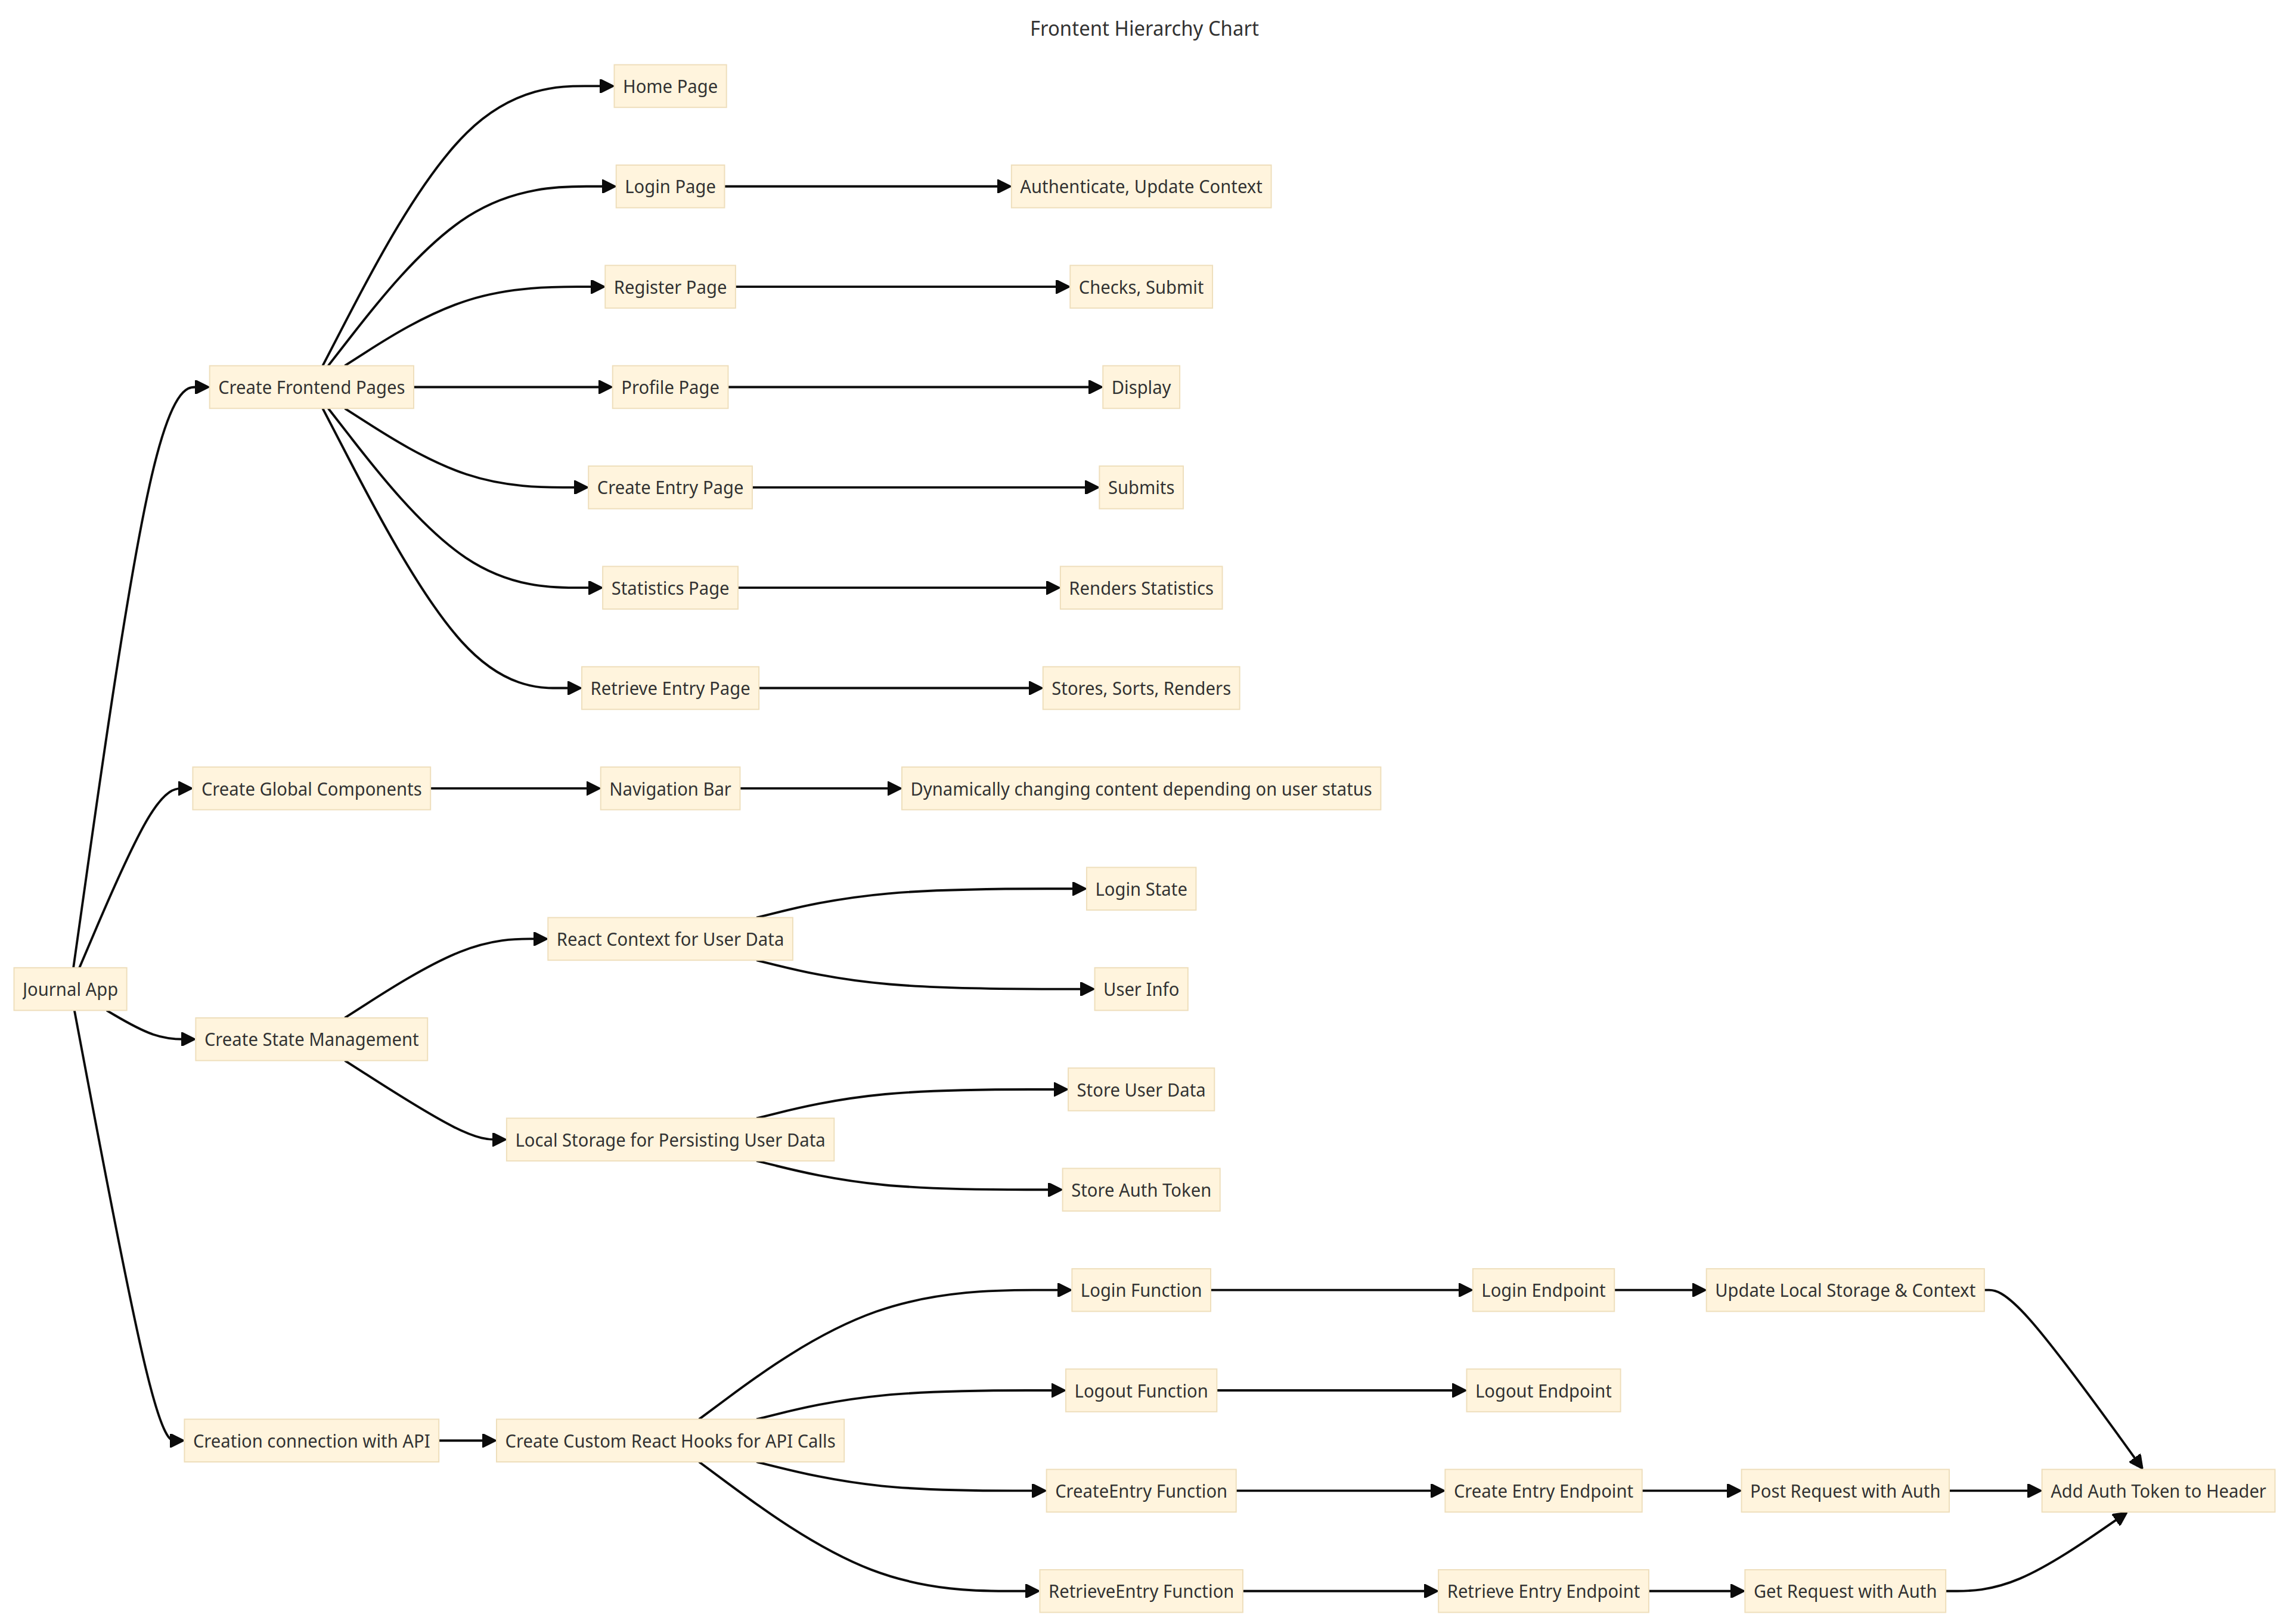
\includegraphics[width=1\linewidth]{Assets/FrontendER.png}
        \caption{Frontend Hierarchy Diagram}
        \label{fig:frontendHD}
    \end{figure}
\end{landscape}

\subsection{Flowchart}
Now, to bring everything together, I have designed a flowchart to depict the flow of operations across the entire system. The overall narrative of the flowchart is that the user interacts with the frontend web pages, and it would trigger functions in the frontend JavaScript code. These functions would perform operations such as making requests to the RESTful API endpoints exposed by the Backend or making changes to the storage in the browser. The front end also manipulates the storage system in the browser while the server handles the database. 

\begin{figure}[h]
    \centering
    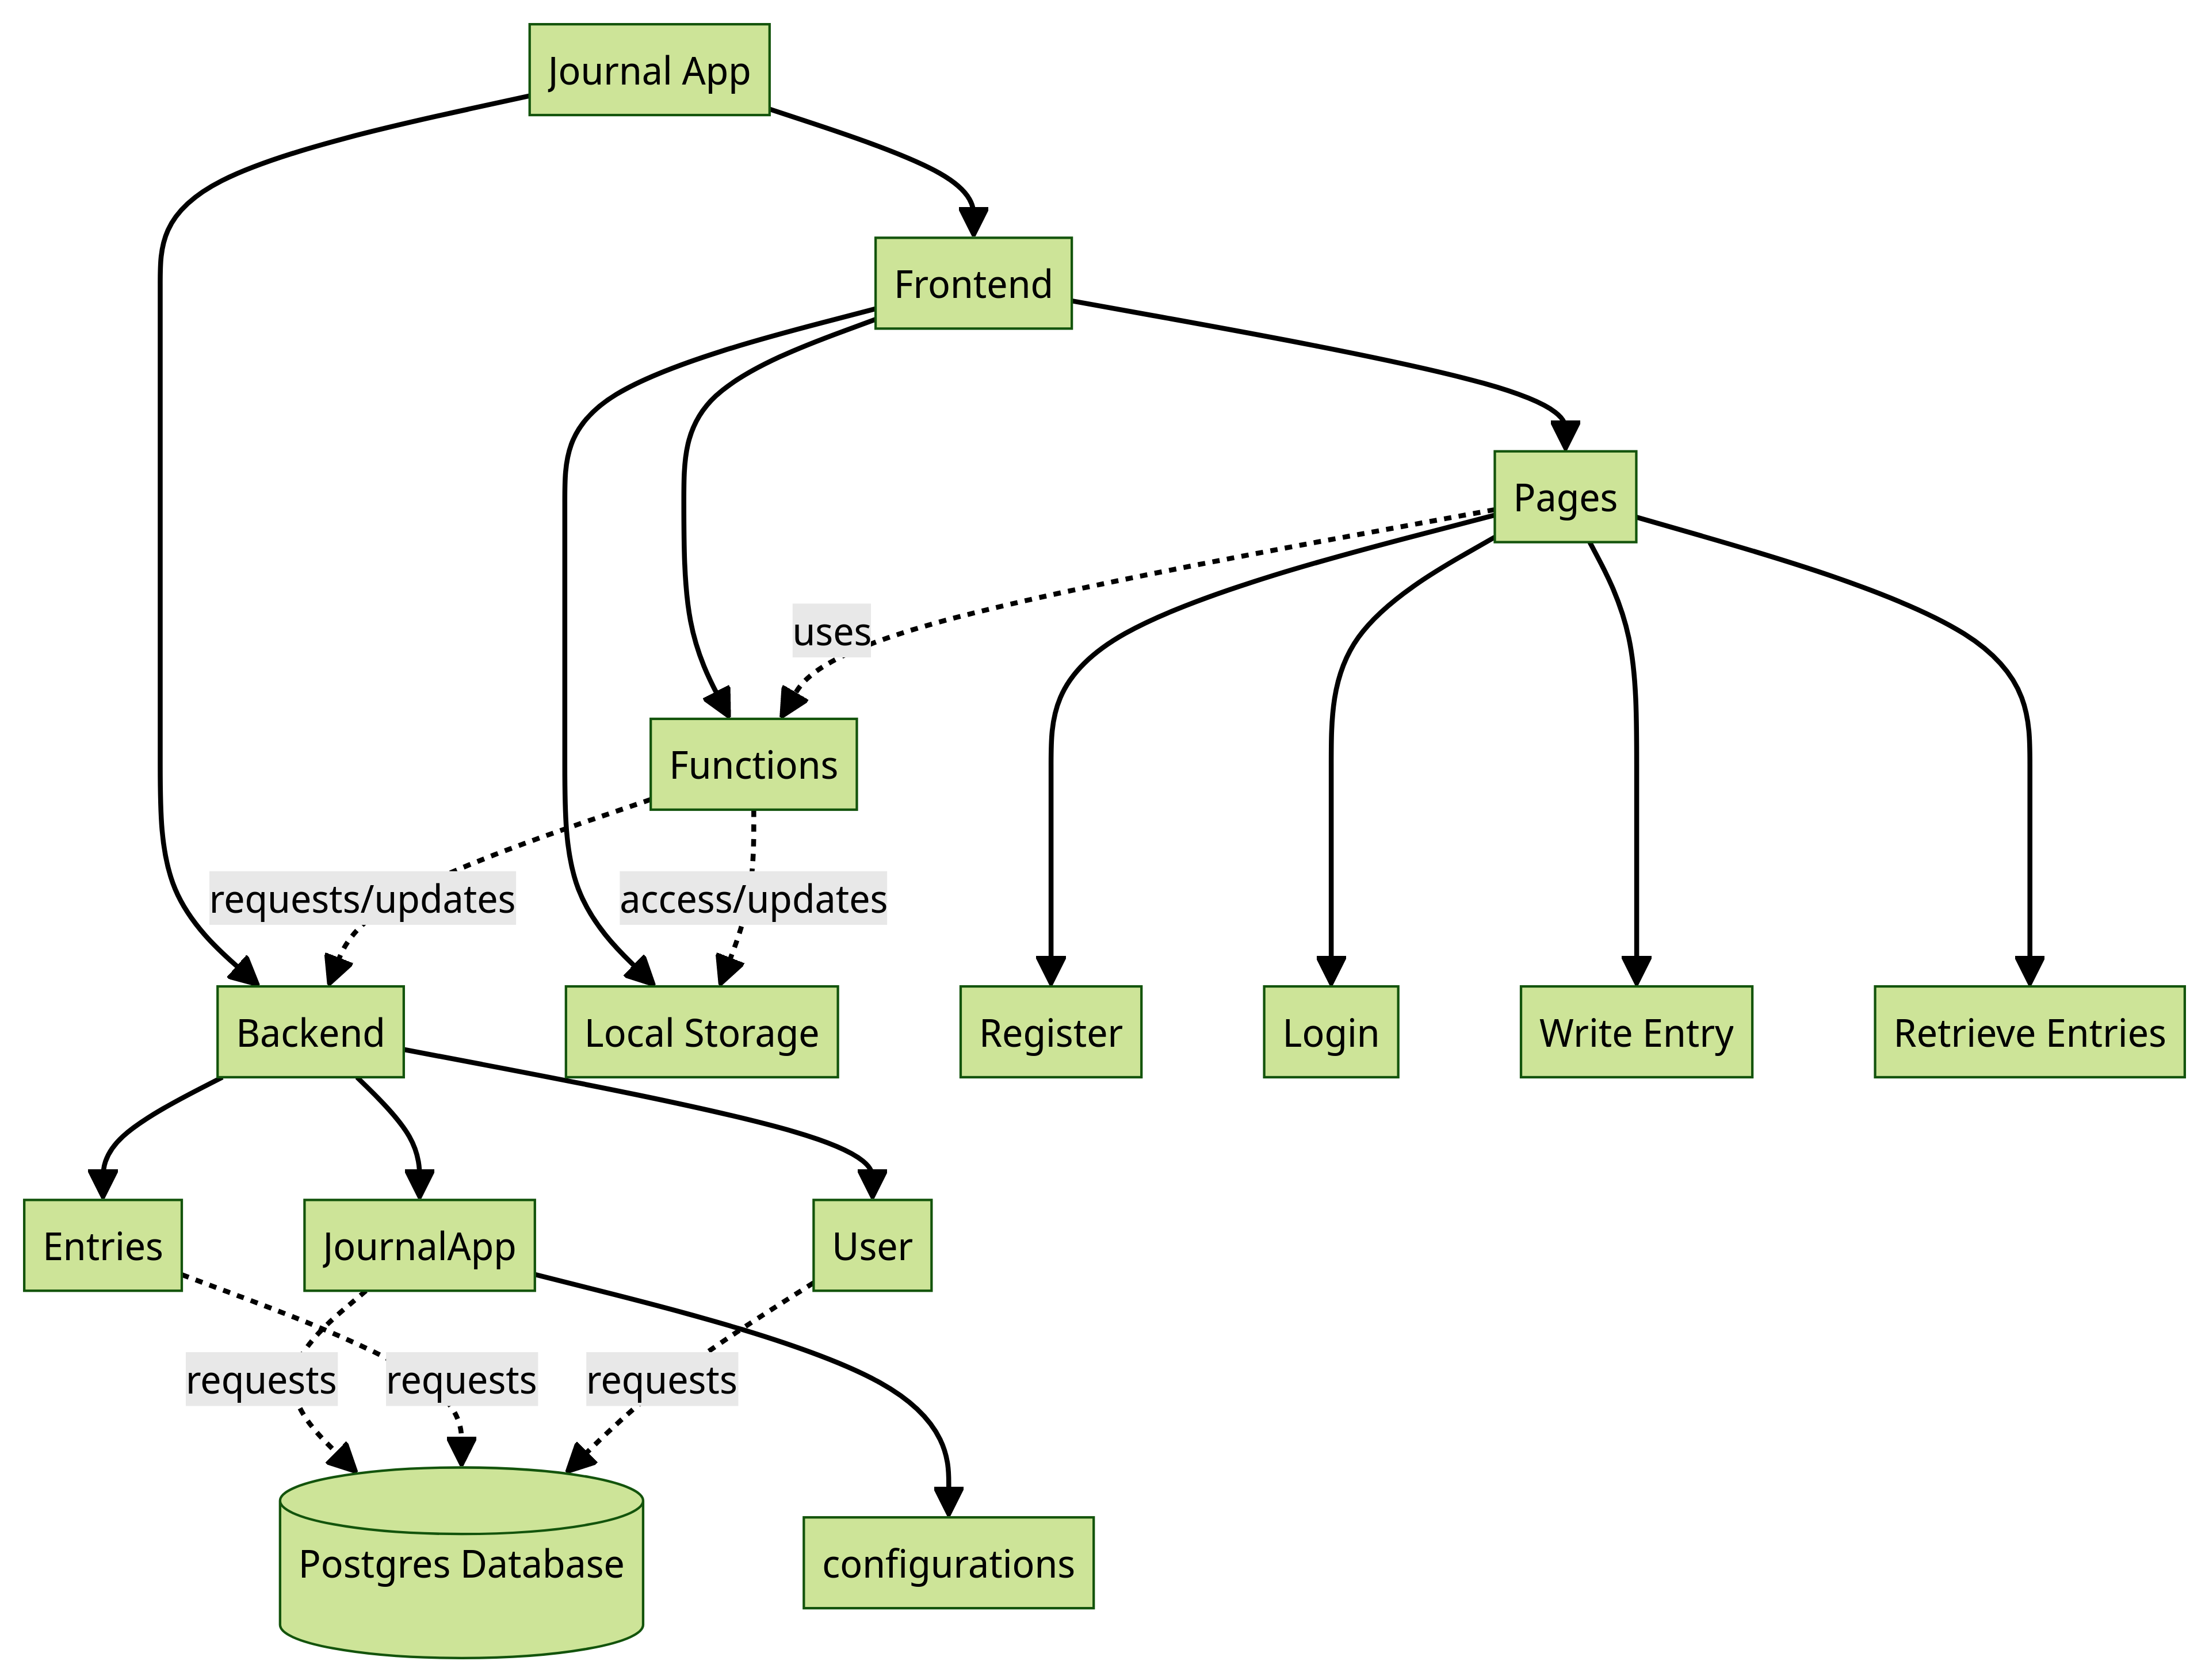
\includegraphics[width=5in]{Assets/Flowchart.png}
    \caption{Flowchart of the System}
    \label{fig:3.3}
\end{figure}

Something to note is that users can only access webpages via HTTP(s) requests (probably through a internet browser). The backend is not intended to be accessed by the user directly. Communication with the server happens internally through private requests. This is a good design practice as it ensures that the server is secure and reduces the risk of attacks by malicious users. 


\section{Data Structures / Data Modelling}
\subsection{Entity Relationship Modelling}
\subsubsection{Storing Data}
In my application, data and the flow of data are integral to the system's overall functionality. I have decided to store the data centrally in a relational database. Central storage ensures reliability, scalability and ease of access of data for me. This is good for my users, who expect their data to be reliably stored and easily accessed.

While it is possible to implement a distributed data storage system for a journal app, I have chosen a centralised approach for simplicity and ease of implementation. Not only is a centralised database more accessible for amateur developers like myself but there are also other reasons why centralised storage is better for my journal app. Keeping entries in a structured place means opportunities to analyse the data. If the user opts in for these features, I could perform sentiment analysis on the user's entries or generate statistics and insights based on their journaling patterns. In fact, Google provides a model for analysing sentiment, which is easily accessible through their API. This is an additional thing I may implement after my project is complete.

I have chosen PostgreSQL as the database management system for my application. Postgres is the most powerful Open-Source option available, and once configured, it provides excellent support for my development environment.

Moreover, If I were to host my application, I could easily connect it to a Postgres database through a cloud provider like Railway.

Looking through the specifications of my journal app, I have identified data that needed to be stored and created a database design in the Third Normal Form.

\subsubsection{Entity Relationship Modelling}
\begin{figure}[!hbt]
    \centering
    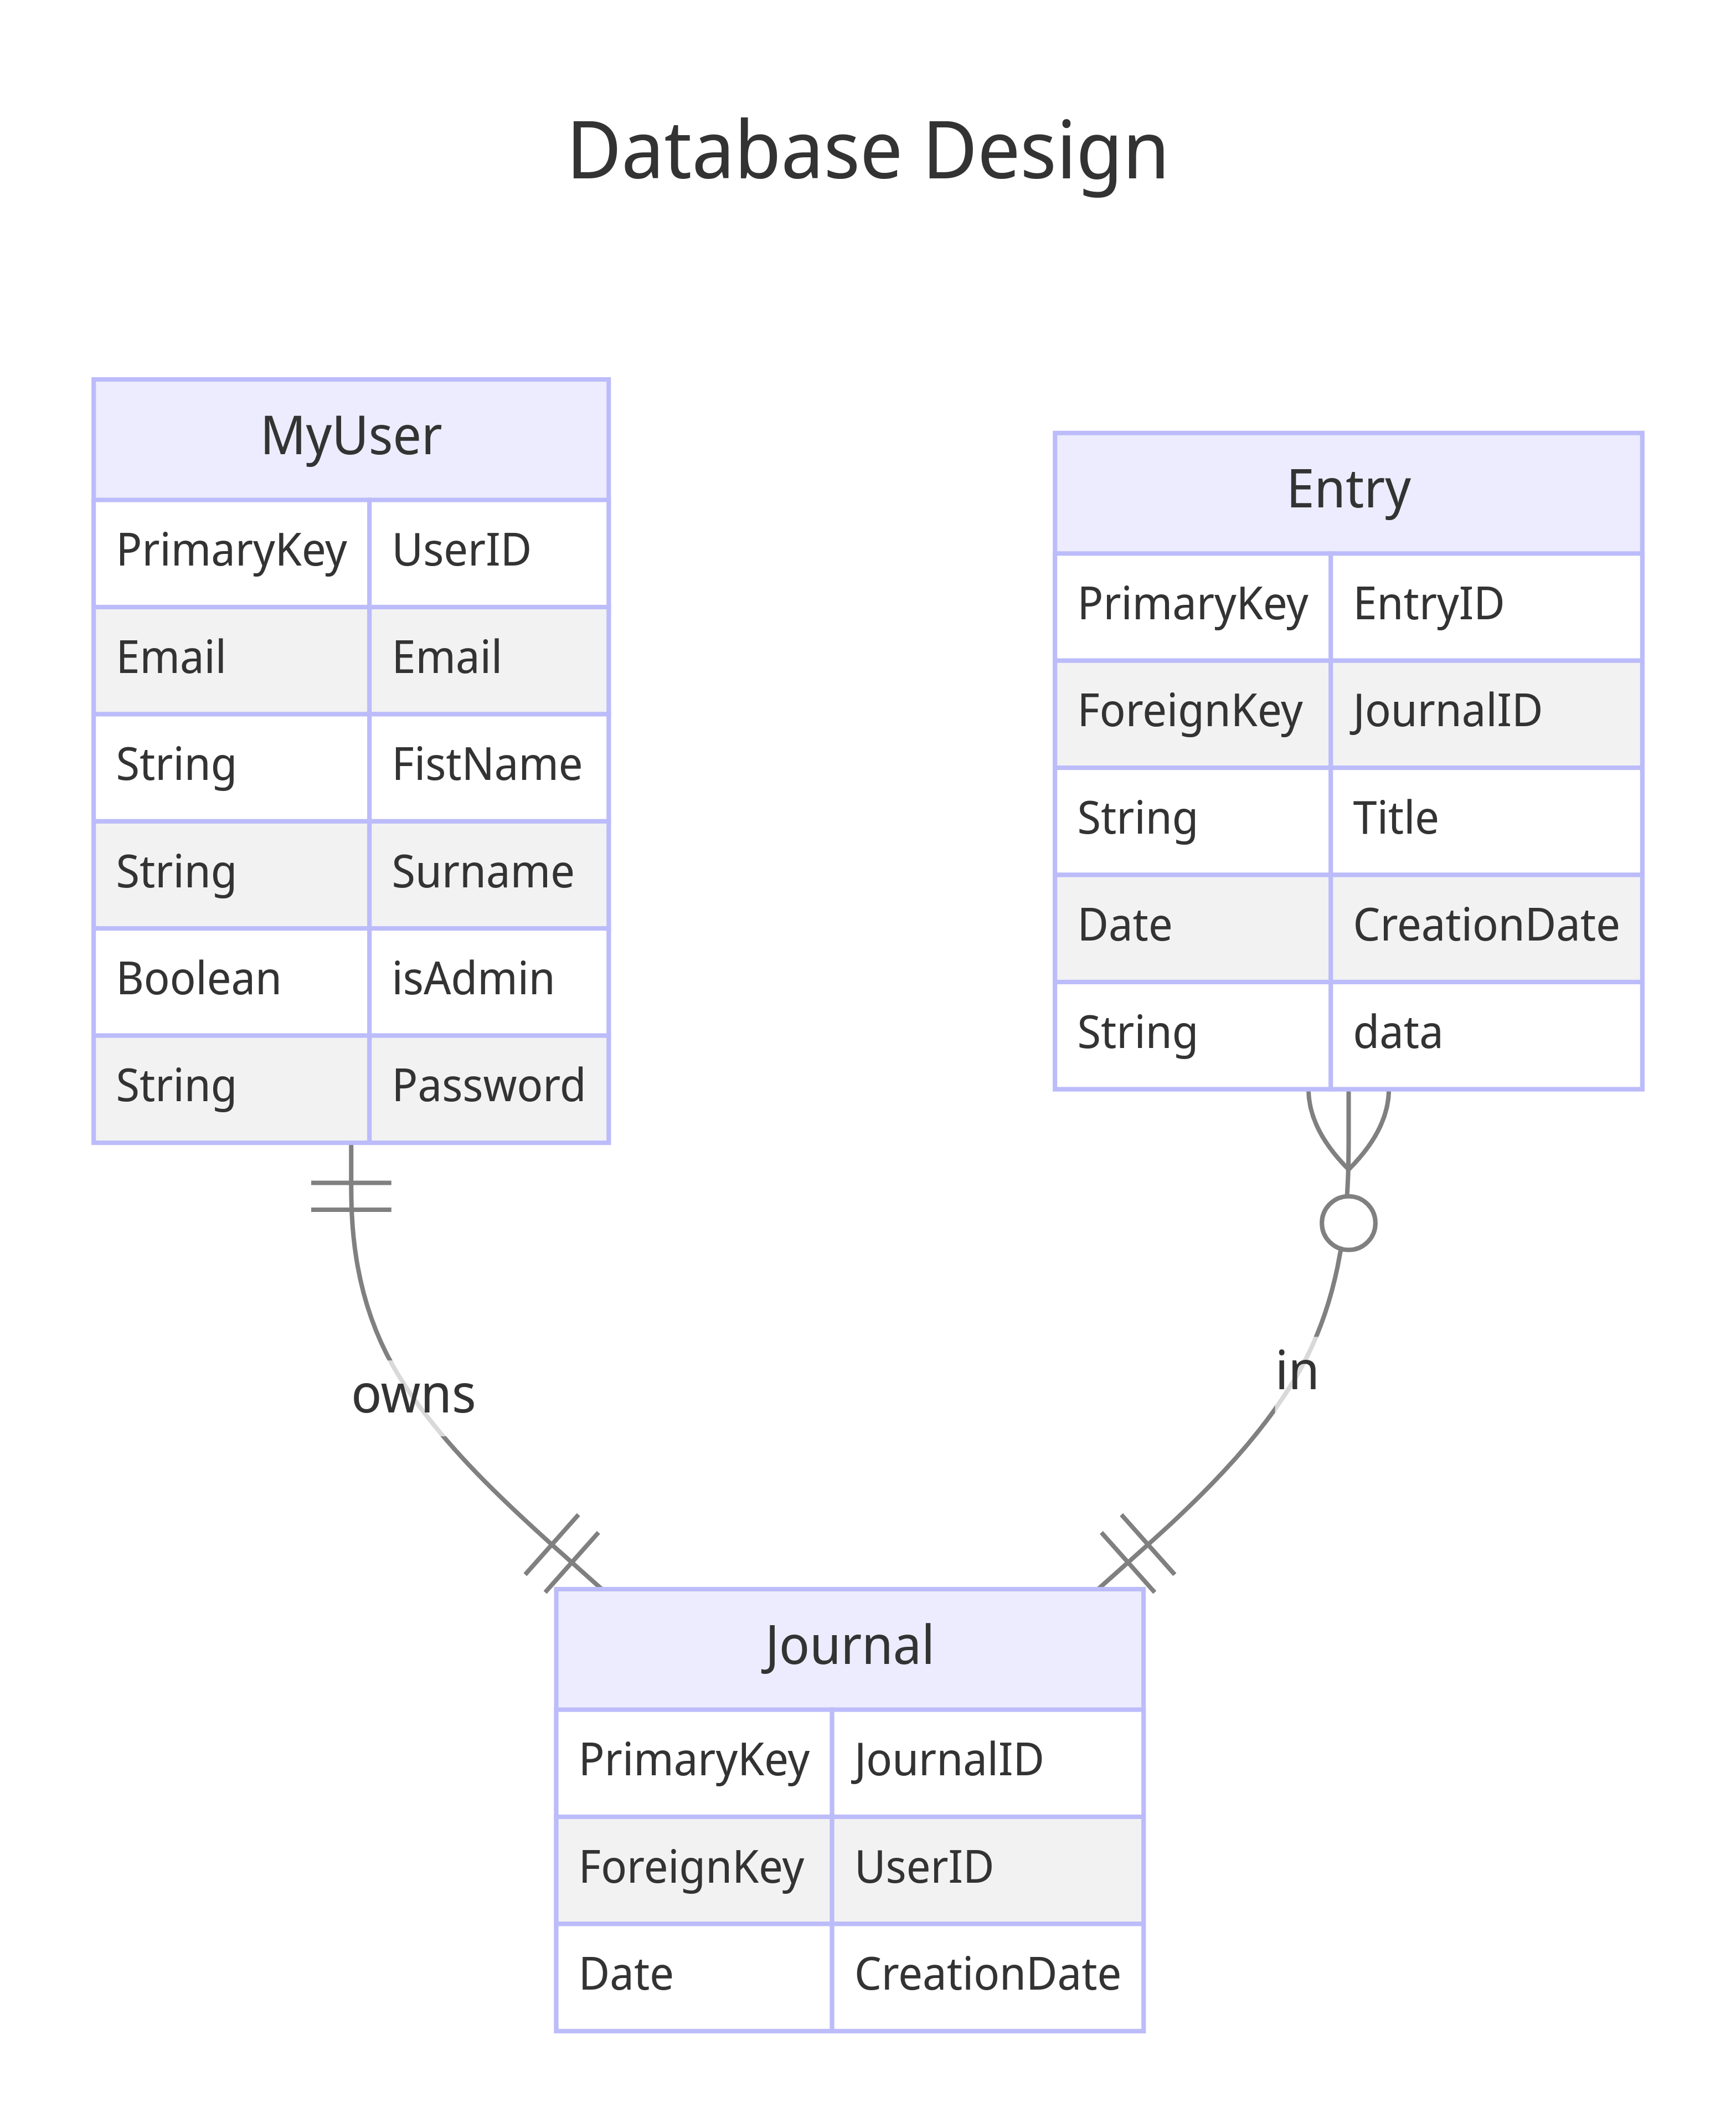
\includegraphics[width=\linewidth]{Assets/Journal Hierarchy ER diagram-2024-03-18-085346.png}
    \caption{Entity Relationship Diagram}
    \label{fig:ER}
\end{figure}



\subsection{External Data Sources}
In a bit of my code I implemented API calls to google cloud natural language API to perform sentiment analysis, it is a method included in the entry class in the backend, it can be used to generate a score for the sentiment of the user represented by a float value. This is just a gimmick feature but not core to the project.

\subsection{OOP Model}
One of the core features of Django is the built-in Object Relation Mapping, which enables me to Model my database using Objects. Initially, I explored writing SQL queries to create my database, but as my project grew in complexity, I realised that to use some powerful features provided by Django, for example, the authentication and the administrator interface, I need to integrate Django's Object Relational Mapping functionalities with my database. With this powerful feature, database schema can be defined using Python classes. Additionally, when it comes to interacting with defined data models, Django provides three ways to interact with the database: the Django ORM, raw SQL queries, and the admin panel. Enabling me to have the best of both worlds, the flexibility of powerful SQL queries and the ease of use of the Django ORM (with the bonus of a GUI interface).


\begin{figure}[!hbt]
    \centering
    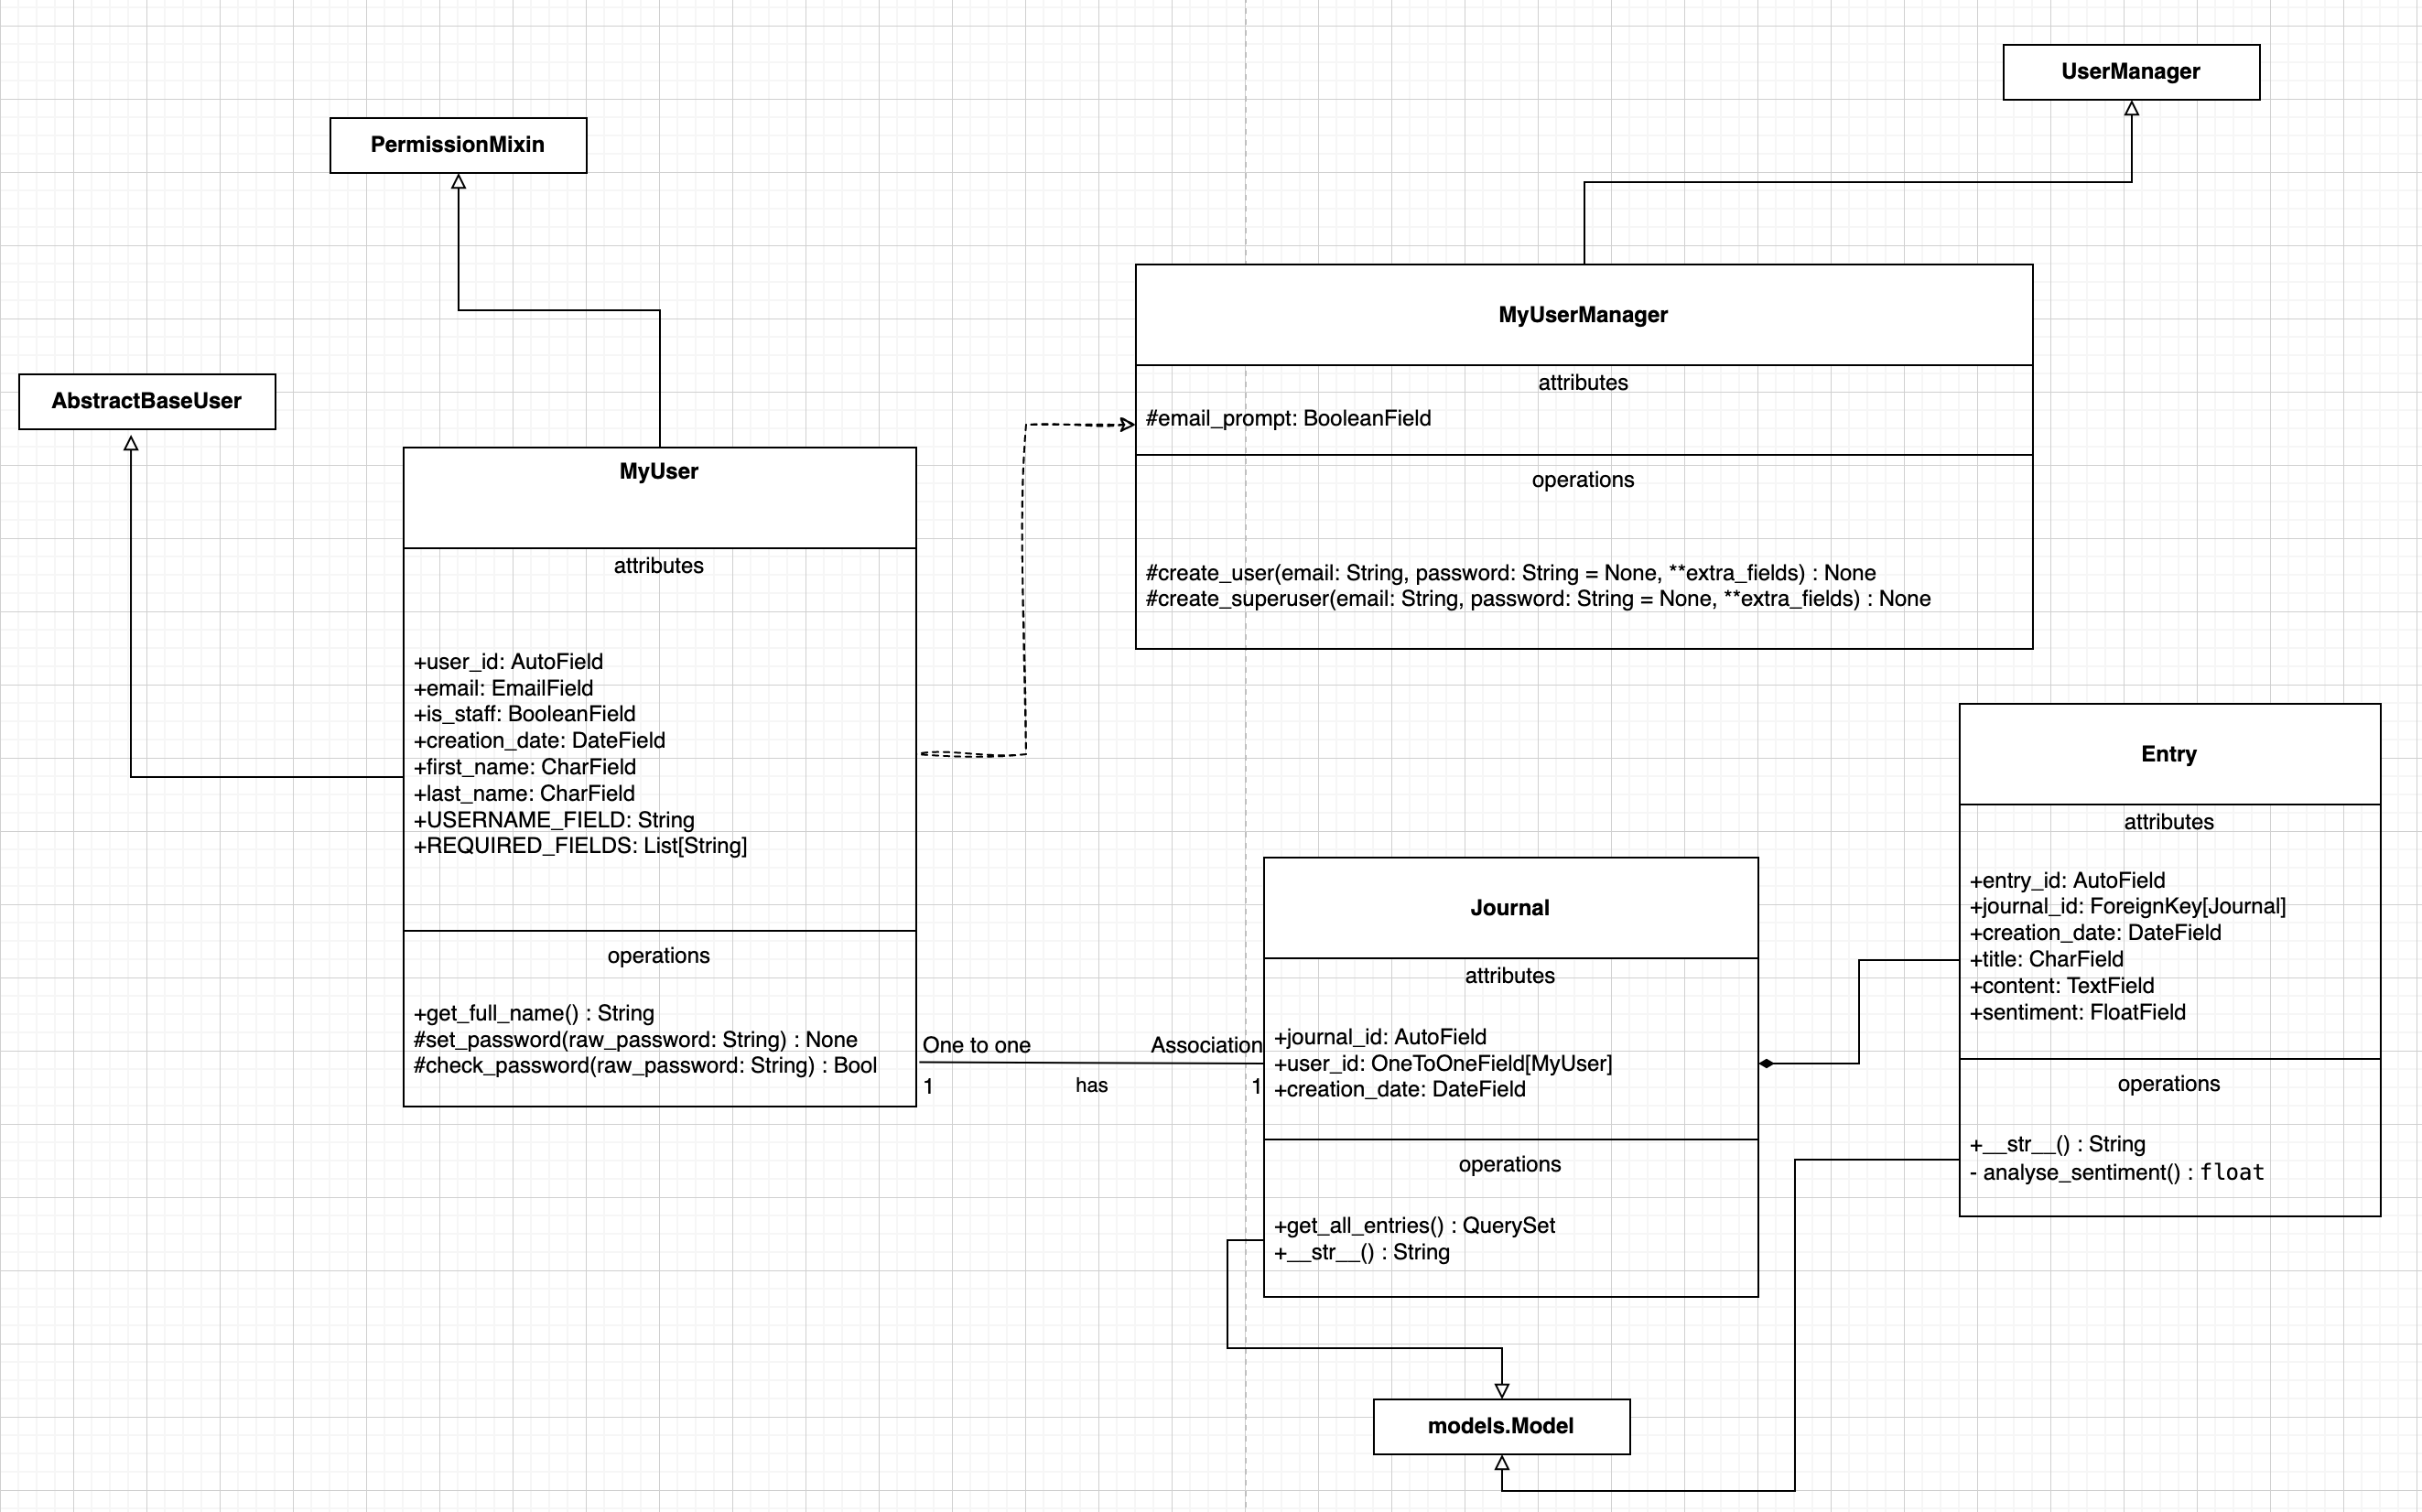
\includegraphics[width=\linewidth]{Assets/UML.png}
    \caption{UML Class Diagram}
    \label{fig:UML}
\end{figure}

\begin{figure}
    \centering
    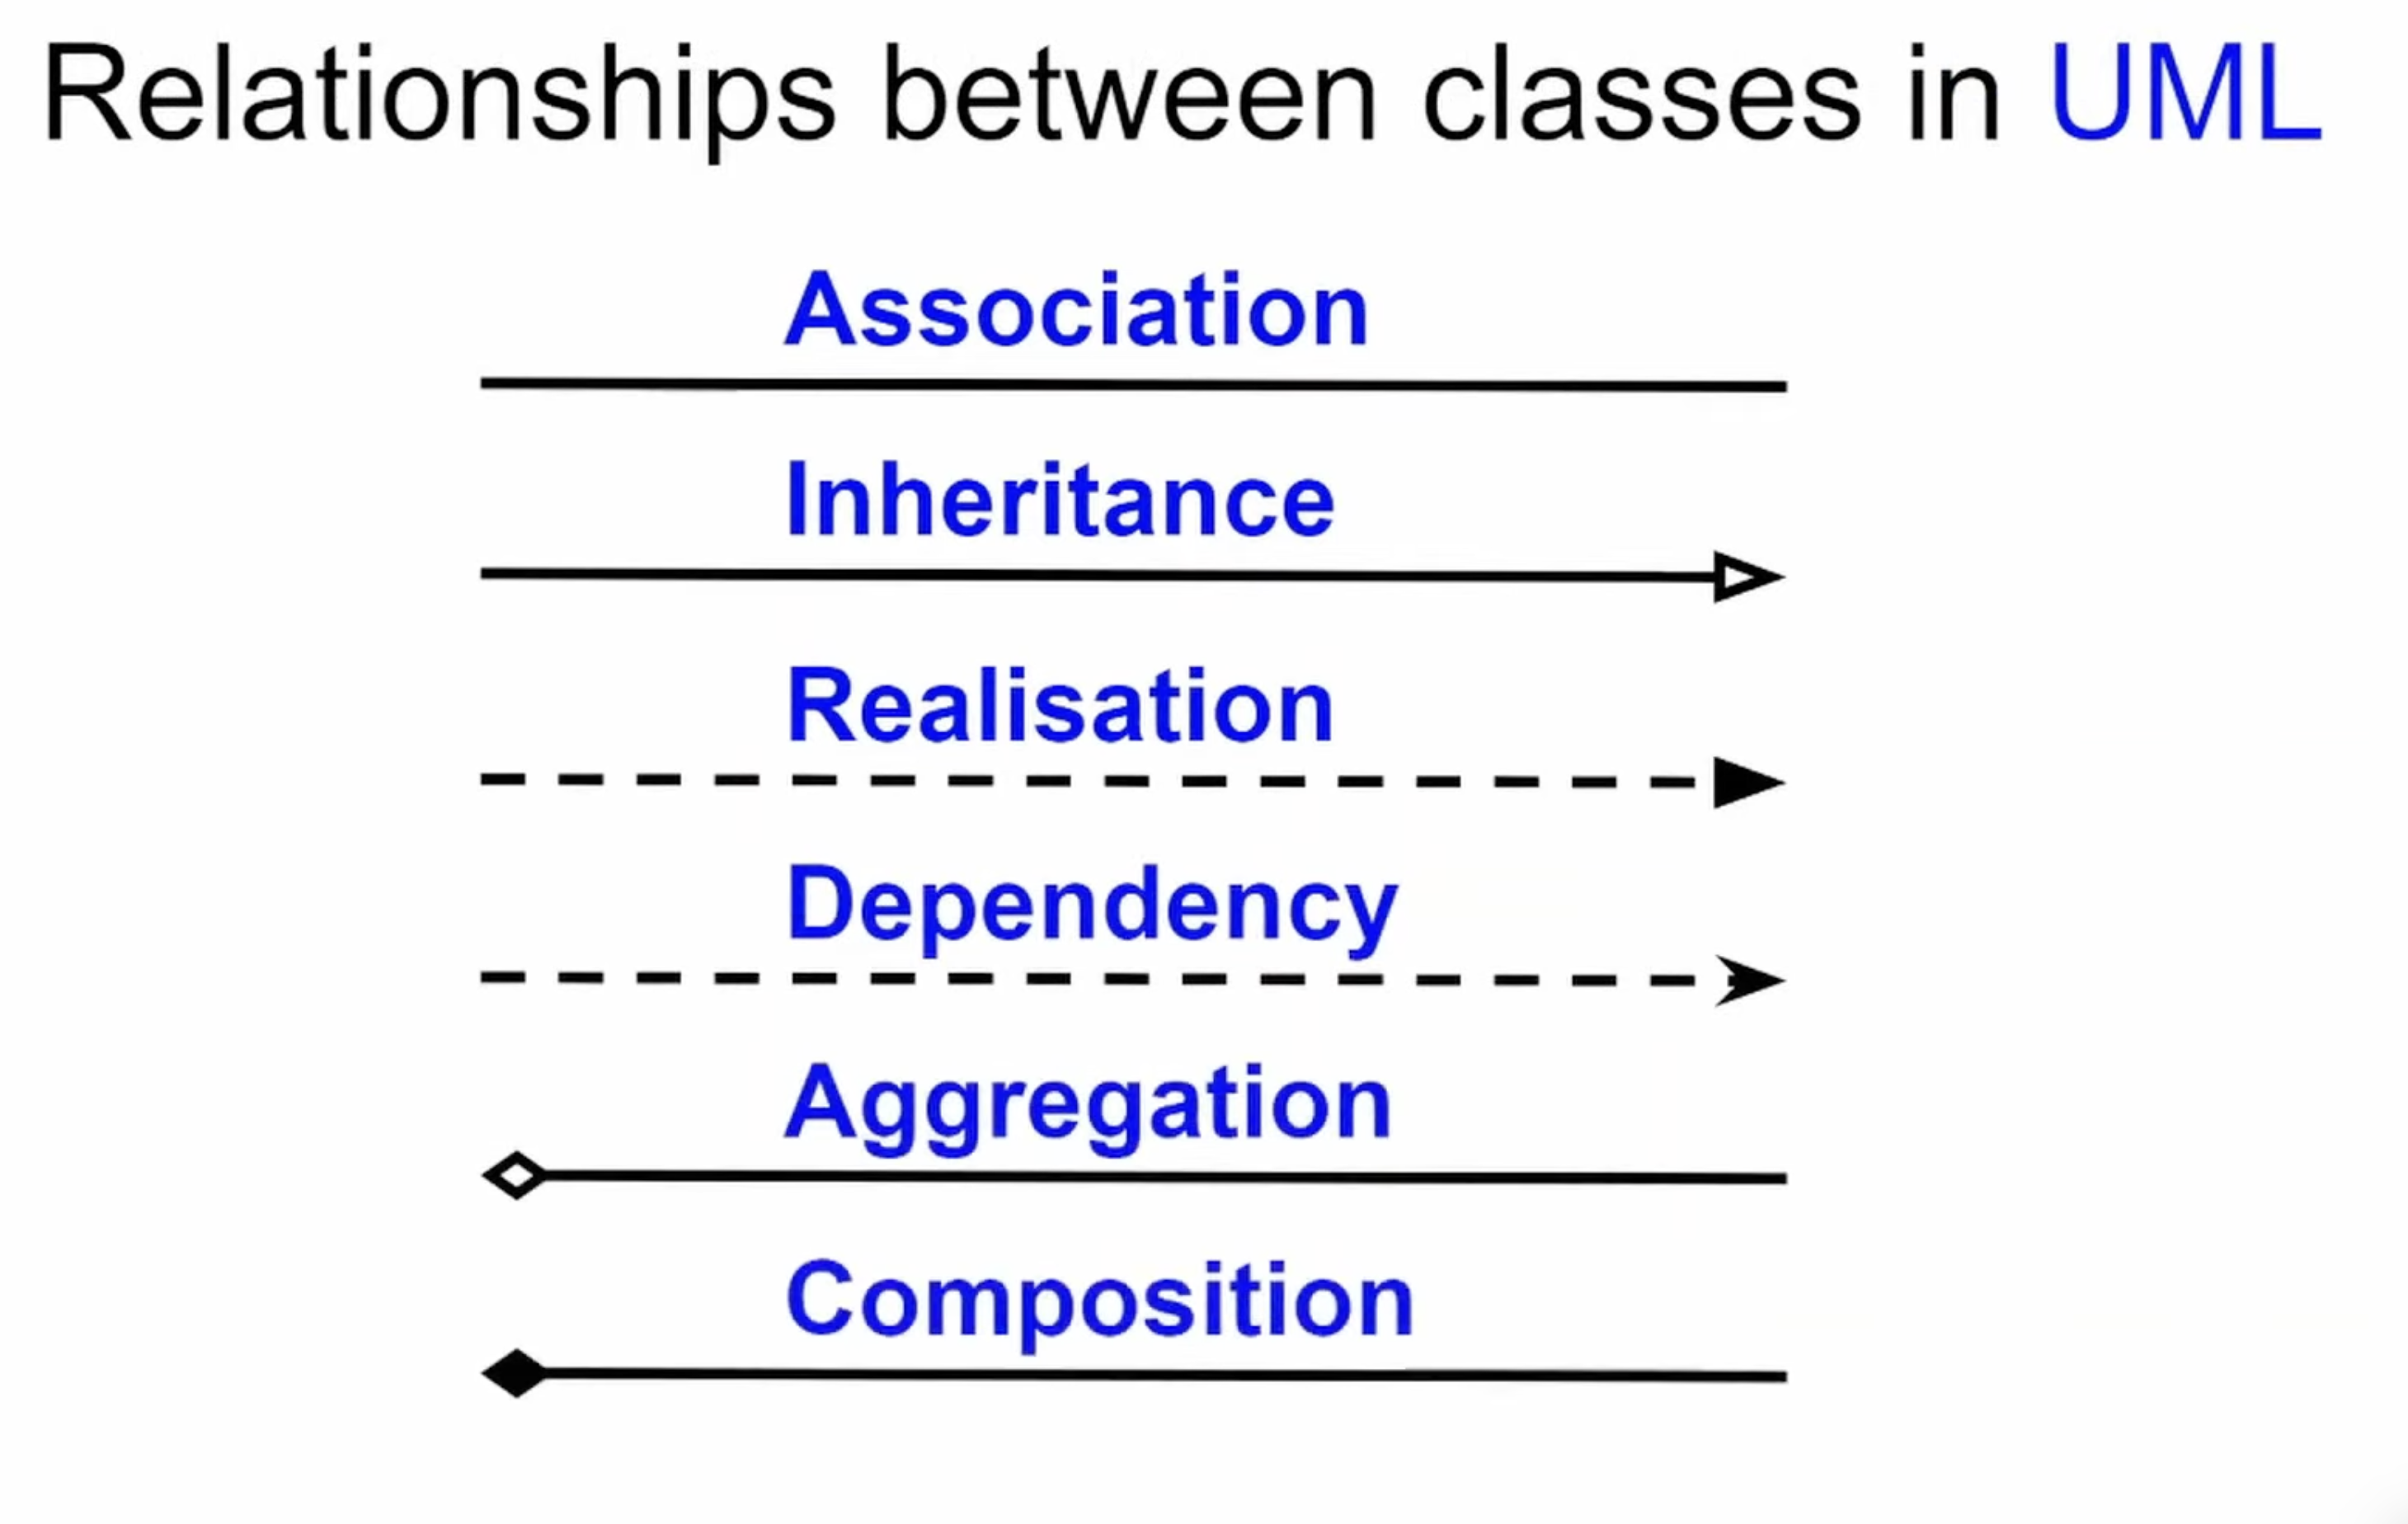
\includegraphics[width=\linewidth]{Assets/UML_keys.png}
    \caption{Keys explaining the arrows in the UML diagram \cite{carnes2021uml}}
\end{figure}

In my models.py file, I have defined several classes that represent different objects in my project:

- MyUser: A class which represents my custom user model in Django, with additional fields and methods tailored to my project's requirements. 

- MyUserManager: A class that manages MyUser class objects, including creating new user instances. MyUser has a dependency on MyUserManager for its functionality.

- Journal: A class representing a journal entry in my project, with fields such as title, content, and date. Journal has a one to one association with MyUser class.

- Entry: A class with a composition relationship with the Journal class, representing a single entry within a journal.

Multiple inheritance is a feature that's not common to all OOP languages since it can lead to potential conflicts and ambiguity in the class hierarchy. In Python, it is supported, and as you can see in the UML diagram, MyUser inherits from AbstractBaseUser and PermissionsMixin. An abstract class is a class that acts as a blueprint for creating a new derived class. I have inherited Django's blueprint for creating users, and I have designed my own user class, which depends on the email field for user registration and login. The second inheritance is from the PermissionsMixin class; this enhances my user class with built-in methods for handling user permissions and authorisation, which is useful. 

Both the Journal and Entry classes are inherited from the Django Model class. This allows me to utilise Django's object relational mapping capabilities to interact with the database smoothly. Entry has a composition relationship with a Journal because an entry is a part of a journal and cannot exist independently. Similarly, the Journal class has a one-to-one association with the MyUser class, indicating that each journal entry is associated with a specific user.

\subsection{Handling JSON}
JSON data are repeatedly used in my project. JSON are in the form of key-value pairs, similar to a dictionary in Python. In my project, I have used JSON data for communication and it is also just a nice way to store other information. One example off the top of my head is that I store the secret key for my application in a secret.json file which I render with python code.

\subsection{Typescript Interface}
Conceptually Typescript interface is very similar to the Object Oriented Principal of Interface. Both are used to layout the "shape" of an object. It allows a form of abstraction and encapsulation in the code, since only the blueprint of the object is defined and also many methods and properties are bundled into one. In my project, Interface is very useful to model the blueprint of the data I am expected to receive from the backend. By defining interfaces, I can guarantee the format of the is as expected which increase the maintainability of the code and reduce the change of unexpected errors.


\section{Algorithms}
In my frontend application, once all the entries are retrieved from my database, in order to improve the experience of the user, I need there to be a way to sort and filter the entries efficiently. While it is possible to create multiple endpoints in my backend application to return the data in multiple ways (e.g. sorted by date, filtered by category), this can result in unnecessary network requests and slower performance. To optimise the sorting and filtering of entries, I can implement an efficient algorithm in my frontend application.

For my purpose I will implement the sorting based on the entry submission date, although it can easily be modified to include other criteria such as the sentiment of the entries.

Choosing an effective algorithm can improve responsiveness of the application and it can especially do so for long term users of the application who might have a large number of entries in their journal.

Sorting algorithms like bubble sort and insertion sort are bad for large datasets since they have a time complexity of O(\(n^2\)) on average. Hence, I will be choosing an efficient sorting algorithm such as Quicksort or Merge Sort, two divide and conquer algorithms, which have a time complexity of $O(n\log{}n)$ on average. Between the two, both offer good performance but they have different implementations and trade offs. I have chosen Quicksort over merge due to the fact that it is In-Place. This means that copies of the list are not created to sort it, making it more efficient in terms of memory.

Writing my own sorting algorithm gives me greater flexibility as I am able to define what is the key that I am deriving my my entries. In my specific case, I have chosen to implement the QuickSort algorithm for sorting the entries based of the creation date of the entry.

Here a simple implementation I have written in Python based on the instructions from OCR A-Level Further Mathematics formula book \cite{ocr2019furthermaths}:
\newpage
\begin{figure}[H]
    \begin{lstlisting}[language=Python]
# my random array
my_array = [3, 6, 8, 10, 1, 2, 1]

def quicksort(array):
    if len(array) == 0:
        return array

    pivot = array[0]
    leftSubarray = []
    rightSubarray = []

    for element in array[1:]:
        # iterating through the array starting from the second element to the end
        if element < pivot:
            leftSubarray.append(element)
        else:
            rightSubarray.append(element)

    leftSubarray = quicksort(leftSubarray)
    rightSubarray = quicksort(rightSubarray)

    return leftSubarray + [pivot] + rightSubarray

# testing the quicksort function
print(quicksort(my_array))
        \end{lstlisting}  
        \caption{QuickSort Python Implementation}

\end{figure}




\section{User Interface}
\subsection{Wireframe Design}

\newpage
% include figures of wireframe designs which takes up the bulk of the page
\begin{figure}[H]
    \centering
    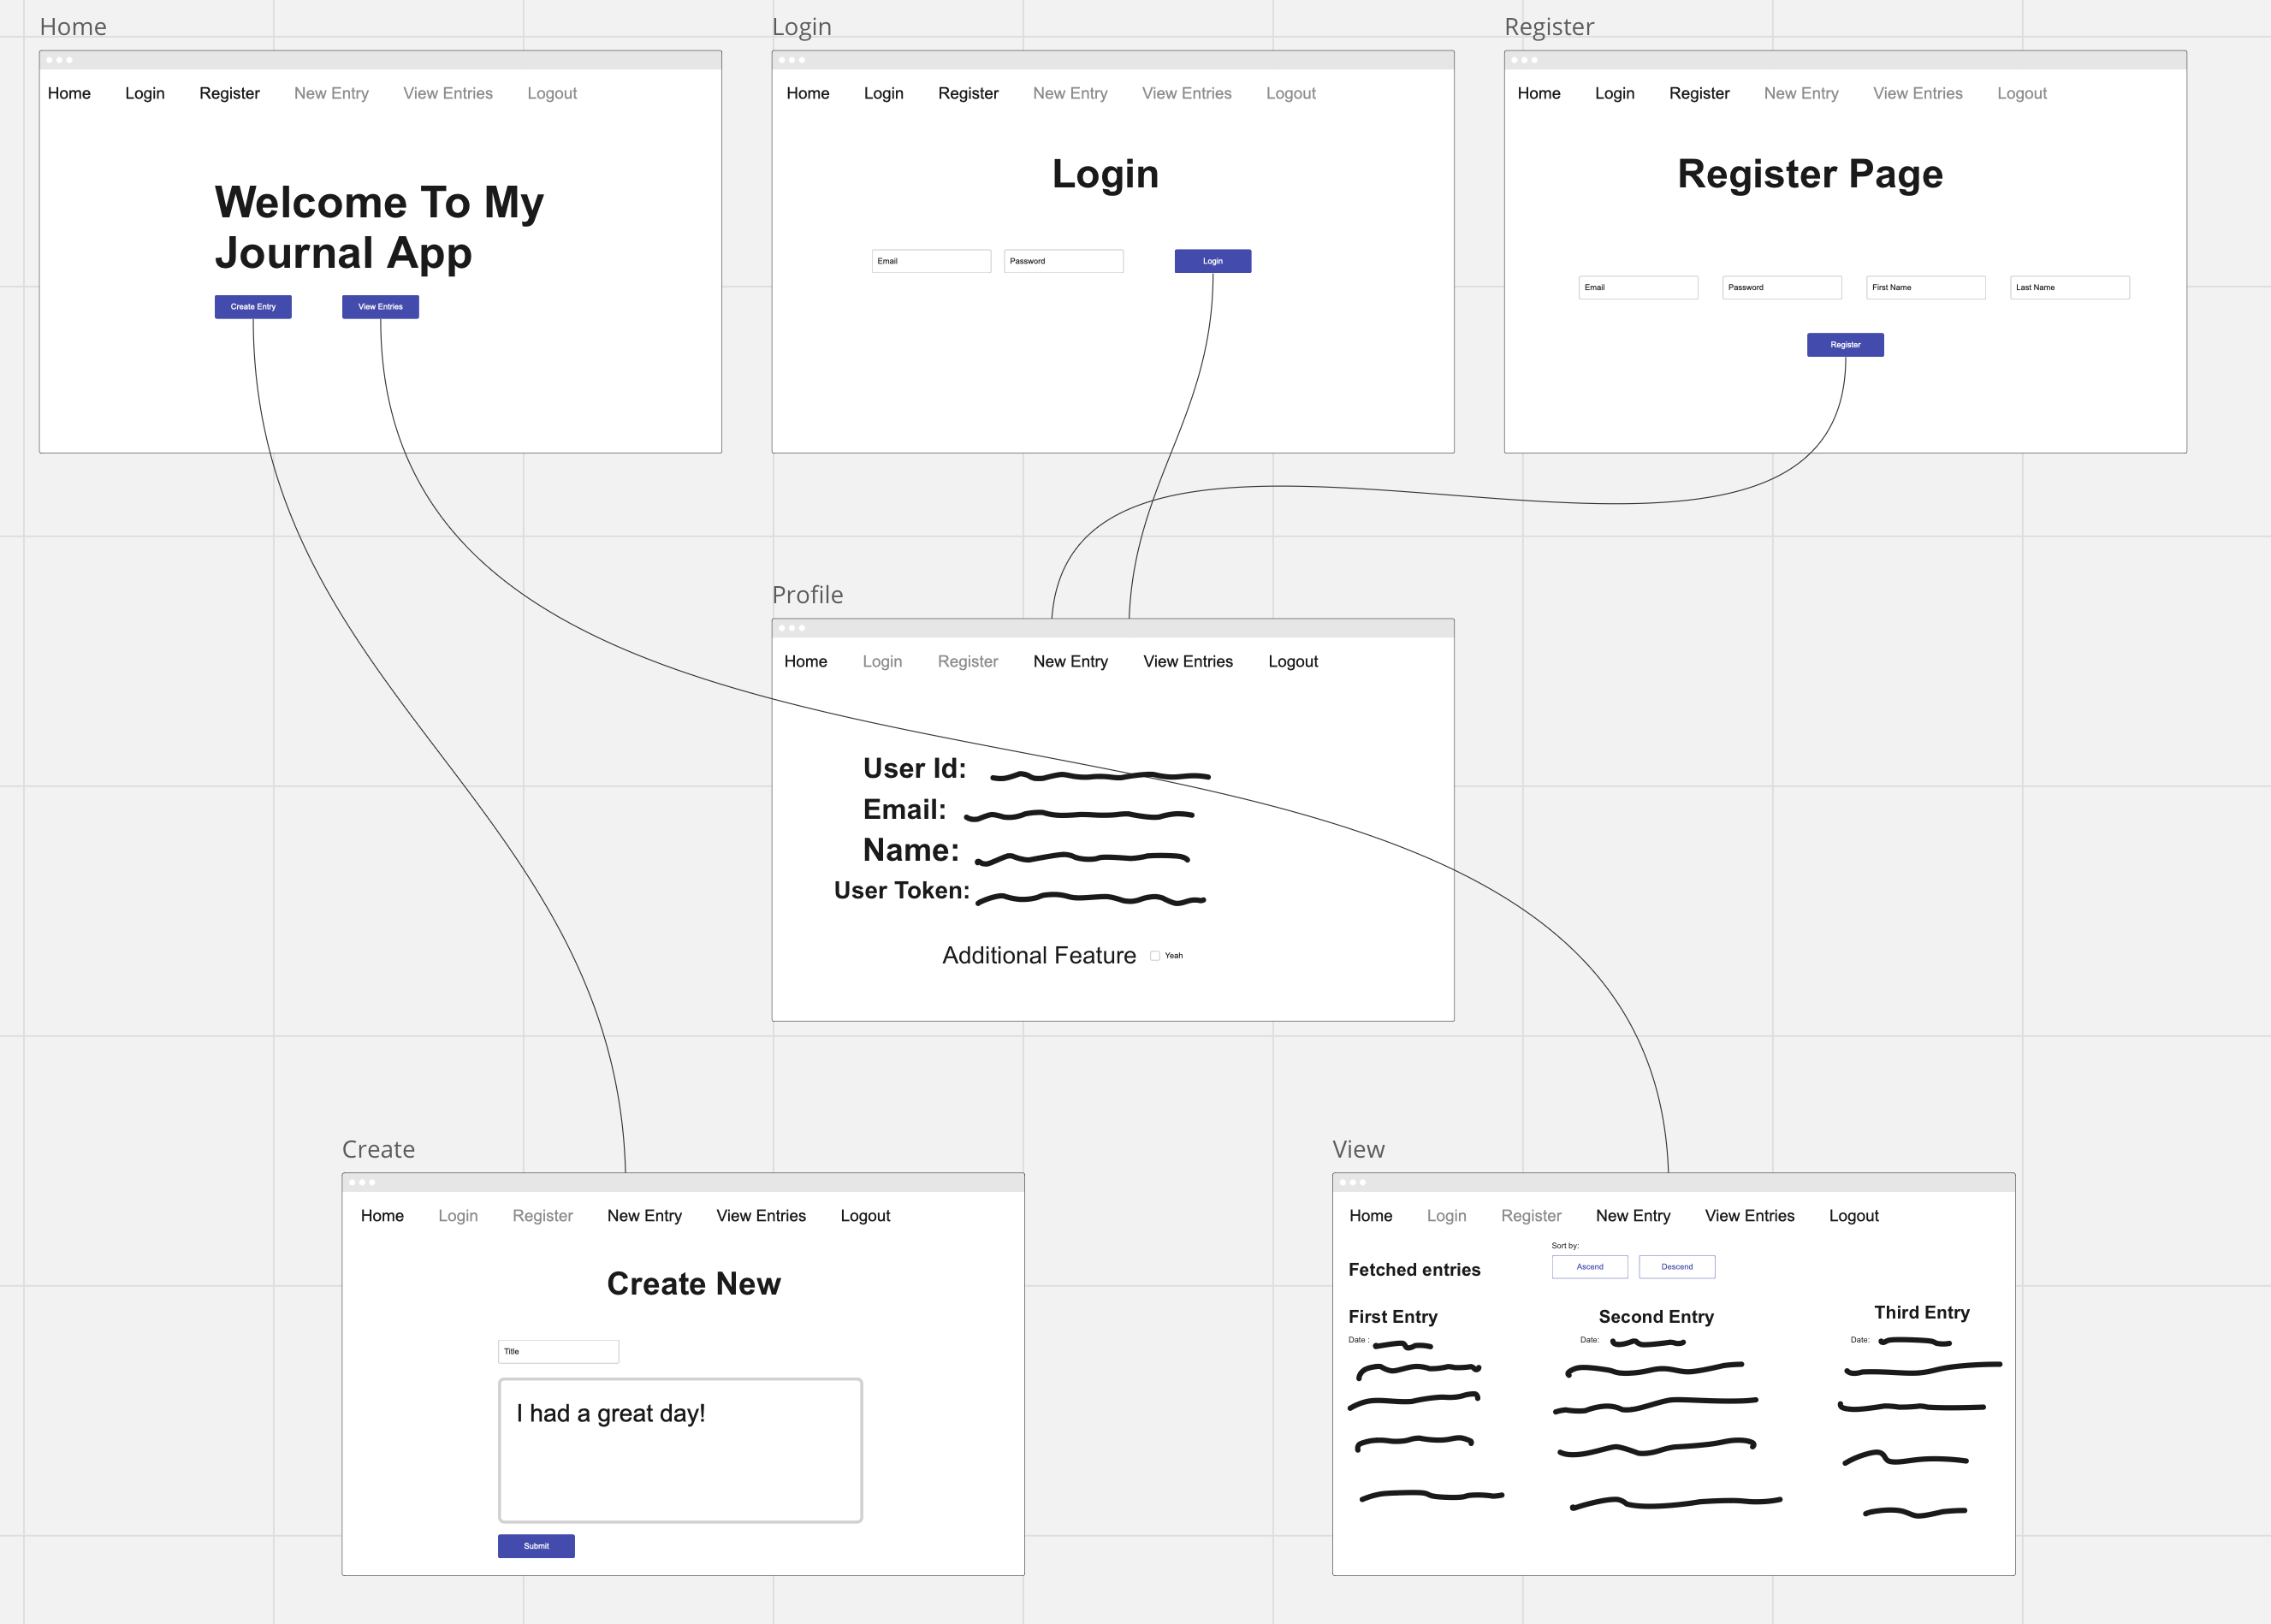
\includegraphics[width=0.8\textwidth]{Assets/all_pages.png}
    \caption{This is an overview of all the screens inside my application, it includes the home page, login page, register page, profile page, create page and view page. There are lines connecting the pages to show the flow of the application. Using the navigation bar at the top, the user can navigate to any page from any page.}
\end{figure}


\begin{figure}[H]
    \centering
    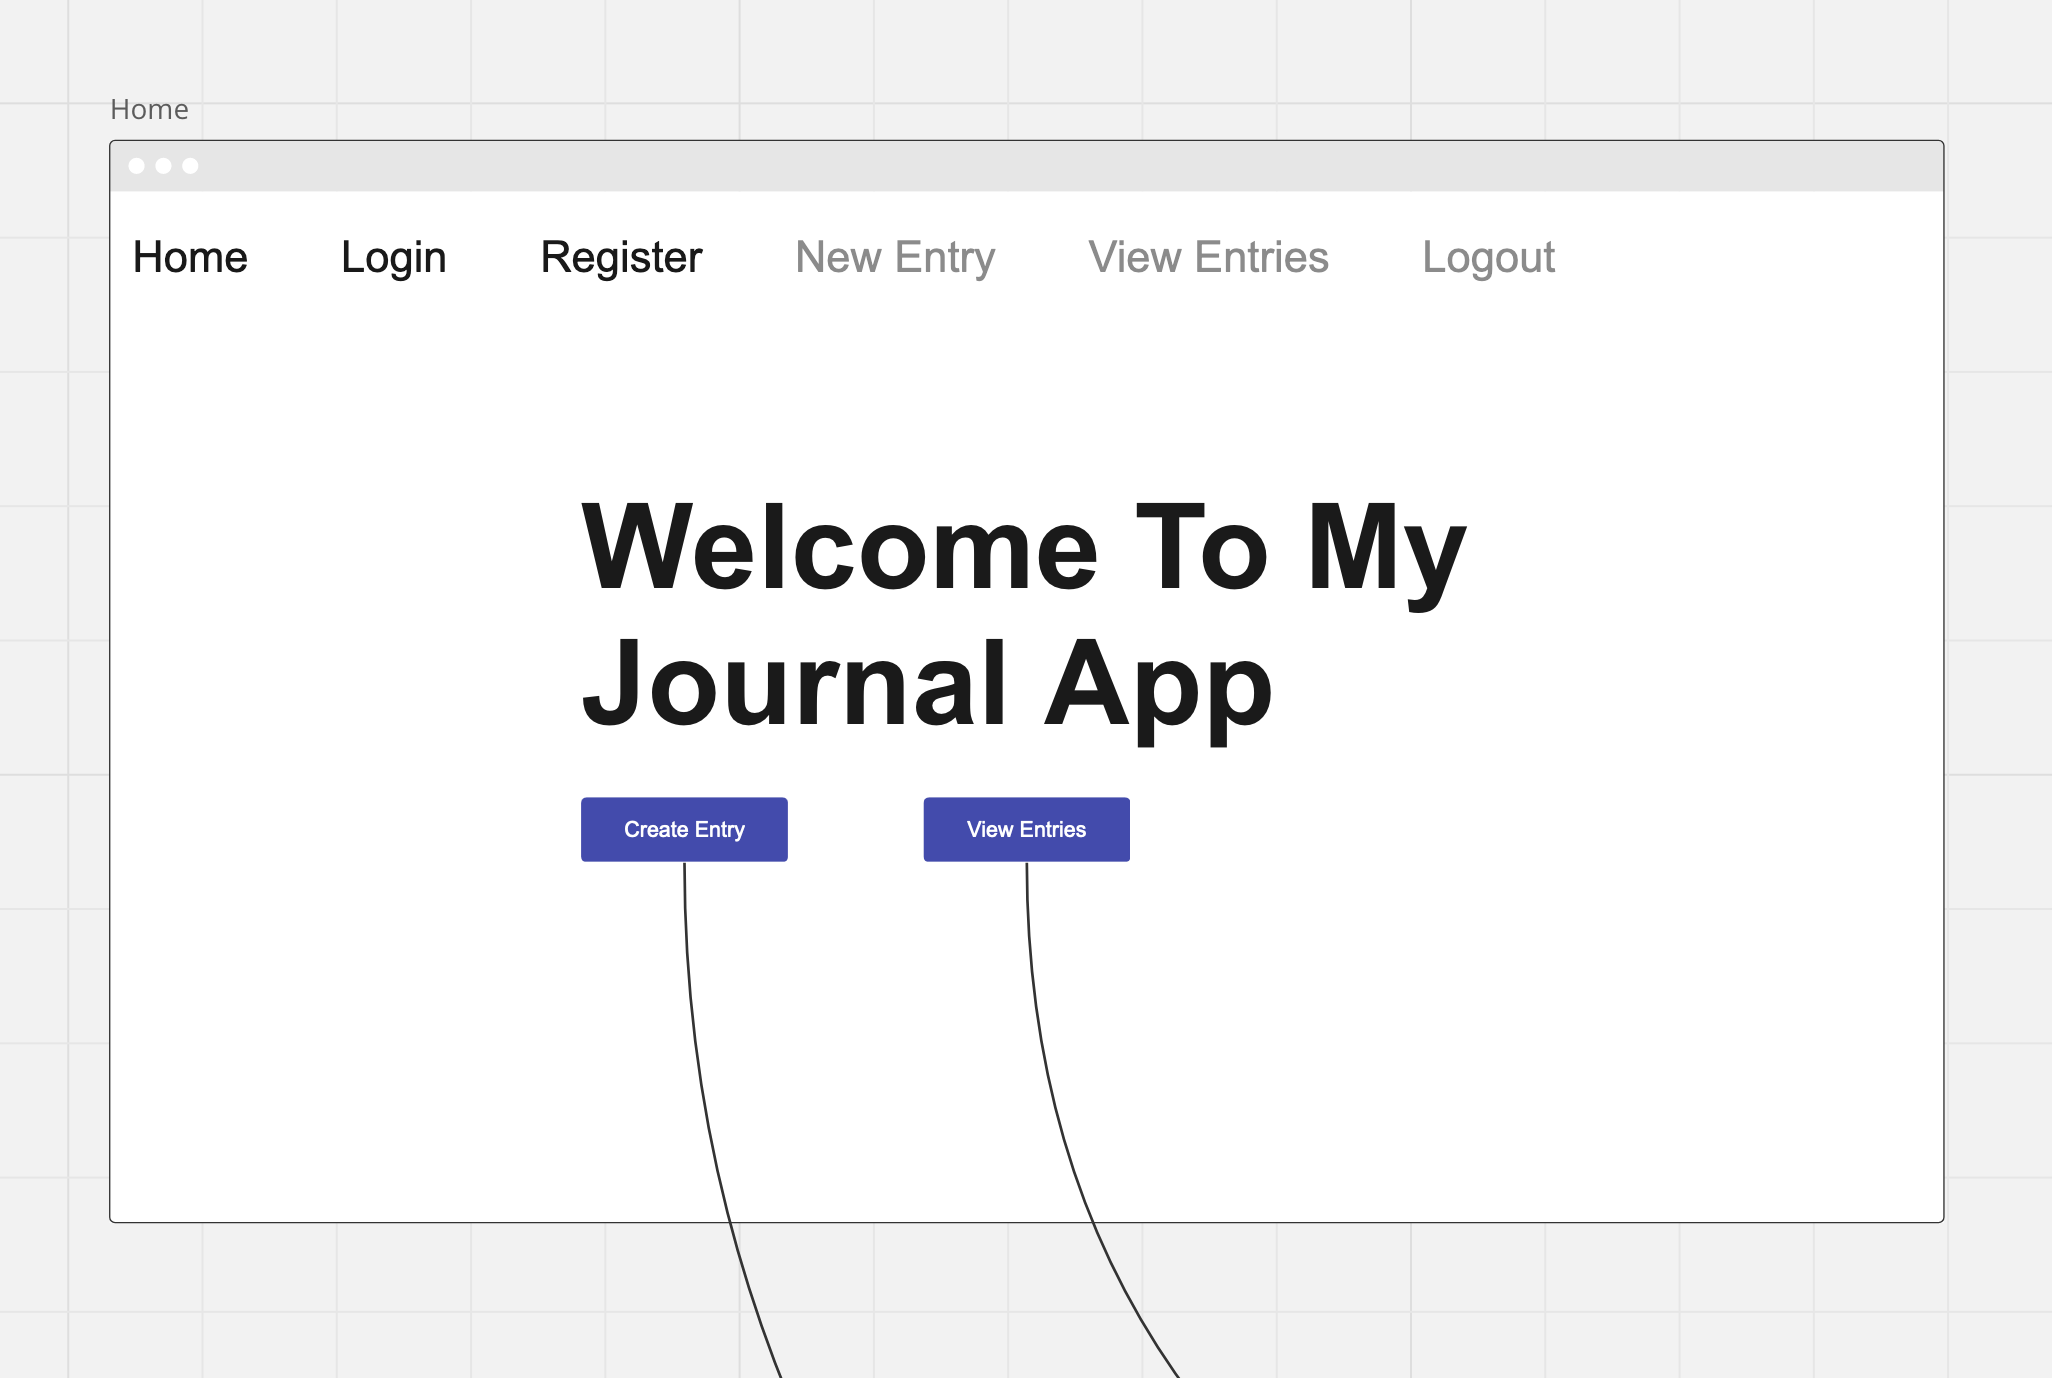
\includegraphics[width=0.7\textwidth]{Assets/home_page.png}
    \caption{The homepage of my application, it includes a navigation bar at the top, a welcome message and buttons for creating and viewing the user's journal entries.}
\end{figure}

\begin{figure}[H]
    \centering
    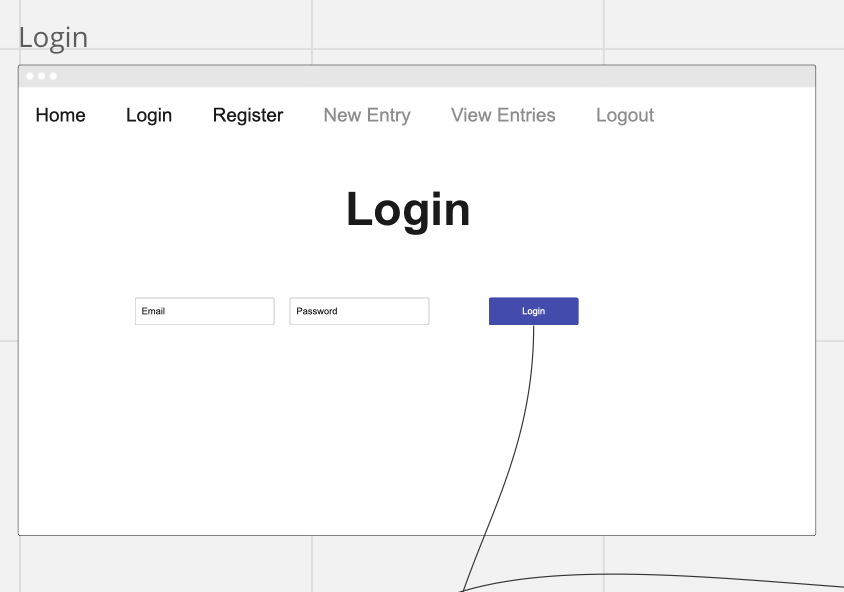
\includegraphics[width=0.7\textwidth]{Assets/login_page.png}
    \caption{The login page of my application, it includes a navigation bar at the top, a form for the user to input their email and password and a button to submit the form. As you can see in the navigation bar, New Entry, View Entries and Logout are all greyed out, this is assuming that the user is not logged in.}
\end{figure}

\begin{figure}[H]
    \centering
    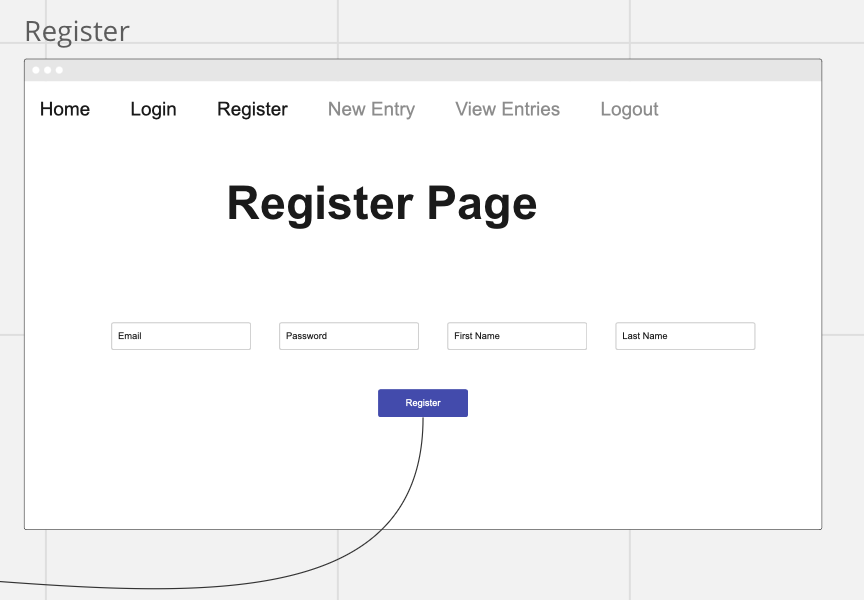
\includegraphics[width=0.8\textwidth]{Assets/register_page.png}
    \caption{Register page is very similar to the login page, it includes a navigation bar at the top, a form for the user inputs as well as the submission button. Registration field requires a couple more fields than the login page.}
\end{figure}

\begin{figure}[H]
    \centering
    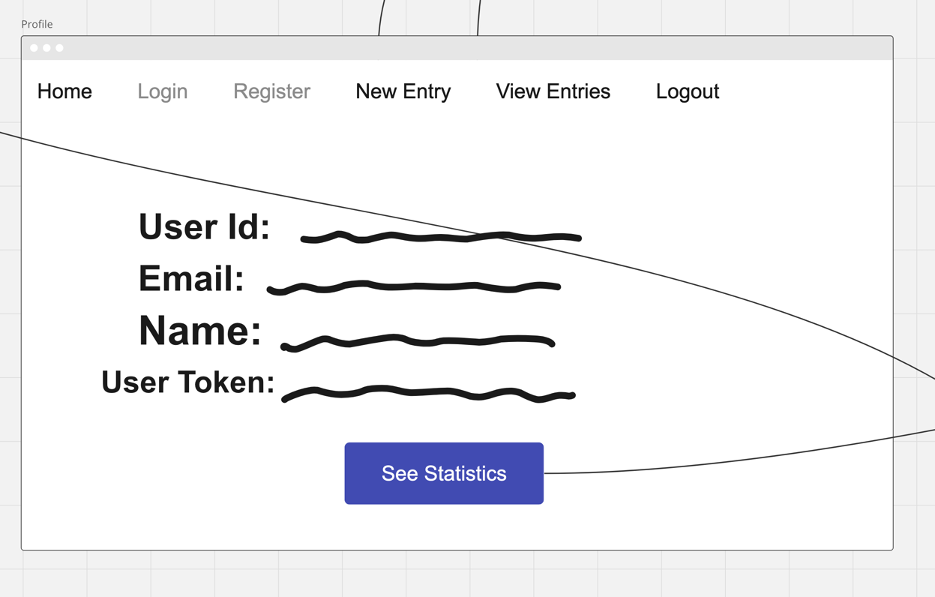
\includegraphics[width=0.8\textwidth]{Assets/profile_page.png}
    \caption{Profile page is where the user can view their profile information, as well as place where they can opt in for some additional features.}
\end{figure}


\begin{figure}[H]
    \centering
    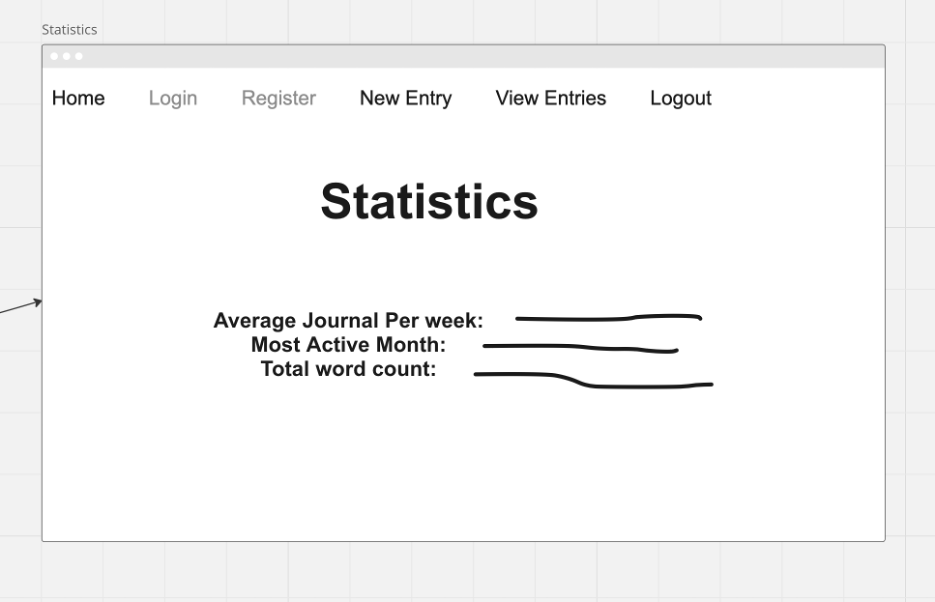
\includegraphics[width=0.8\textwidth]{Assets/statistics_page.png}
    \caption{Statistics page is where the user can view statistics based on their journal entries pattern.}
\end{figure}


\begin{figure}[H]
    \centering
    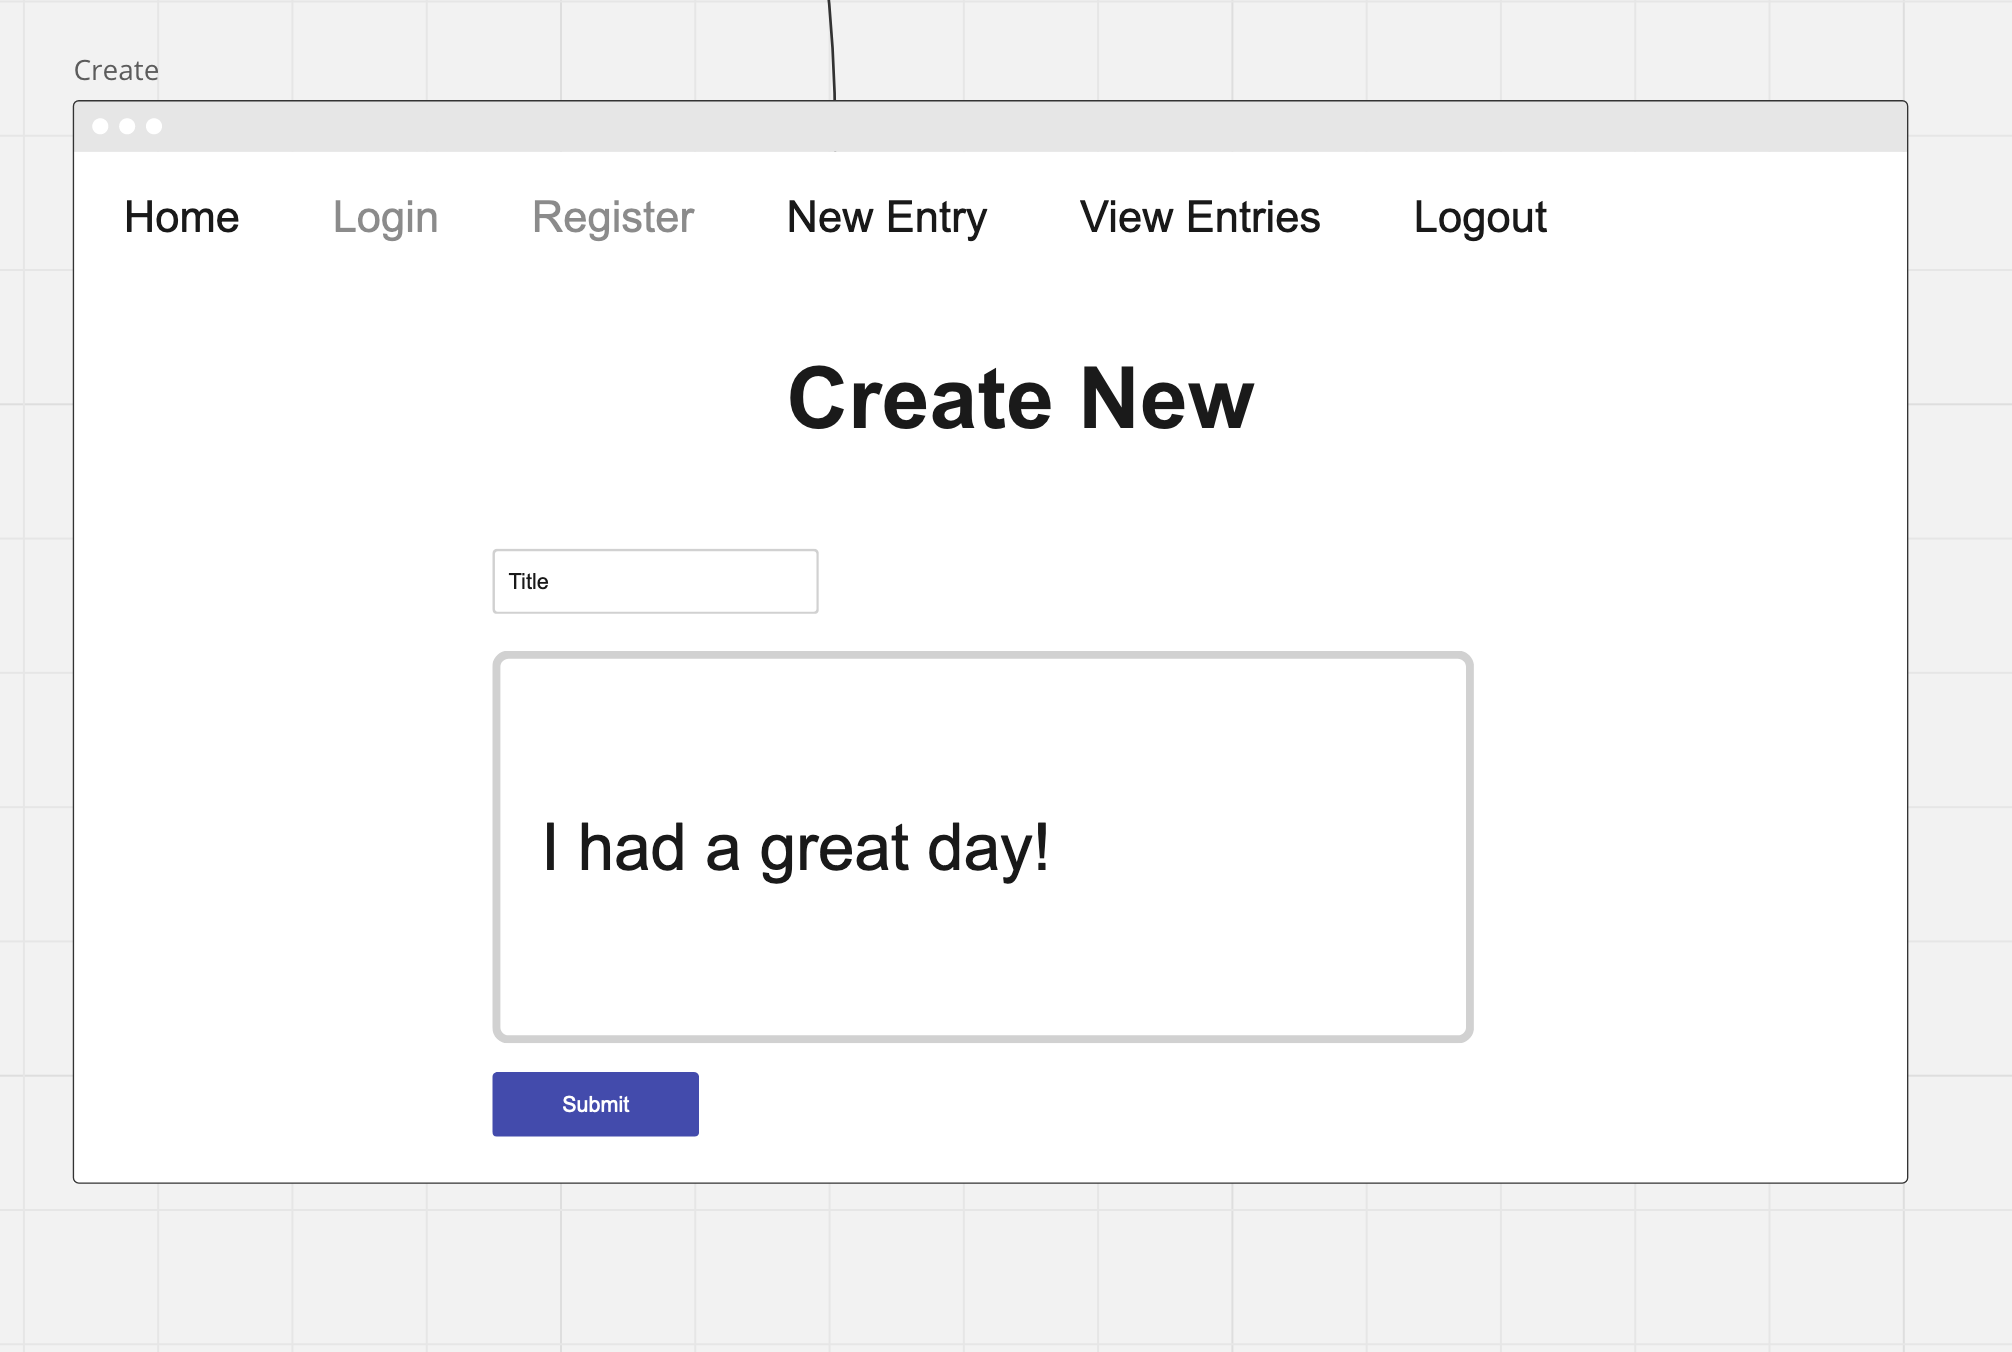
\includegraphics[width=0.8\textwidth]{Assets/create_page.png}
    \caption{Create page is where the user can create a new journal entry. It includes a form for the user to input the title and content of the entry.}
\end{figure}

\begin{figure}[H]
    \centering
    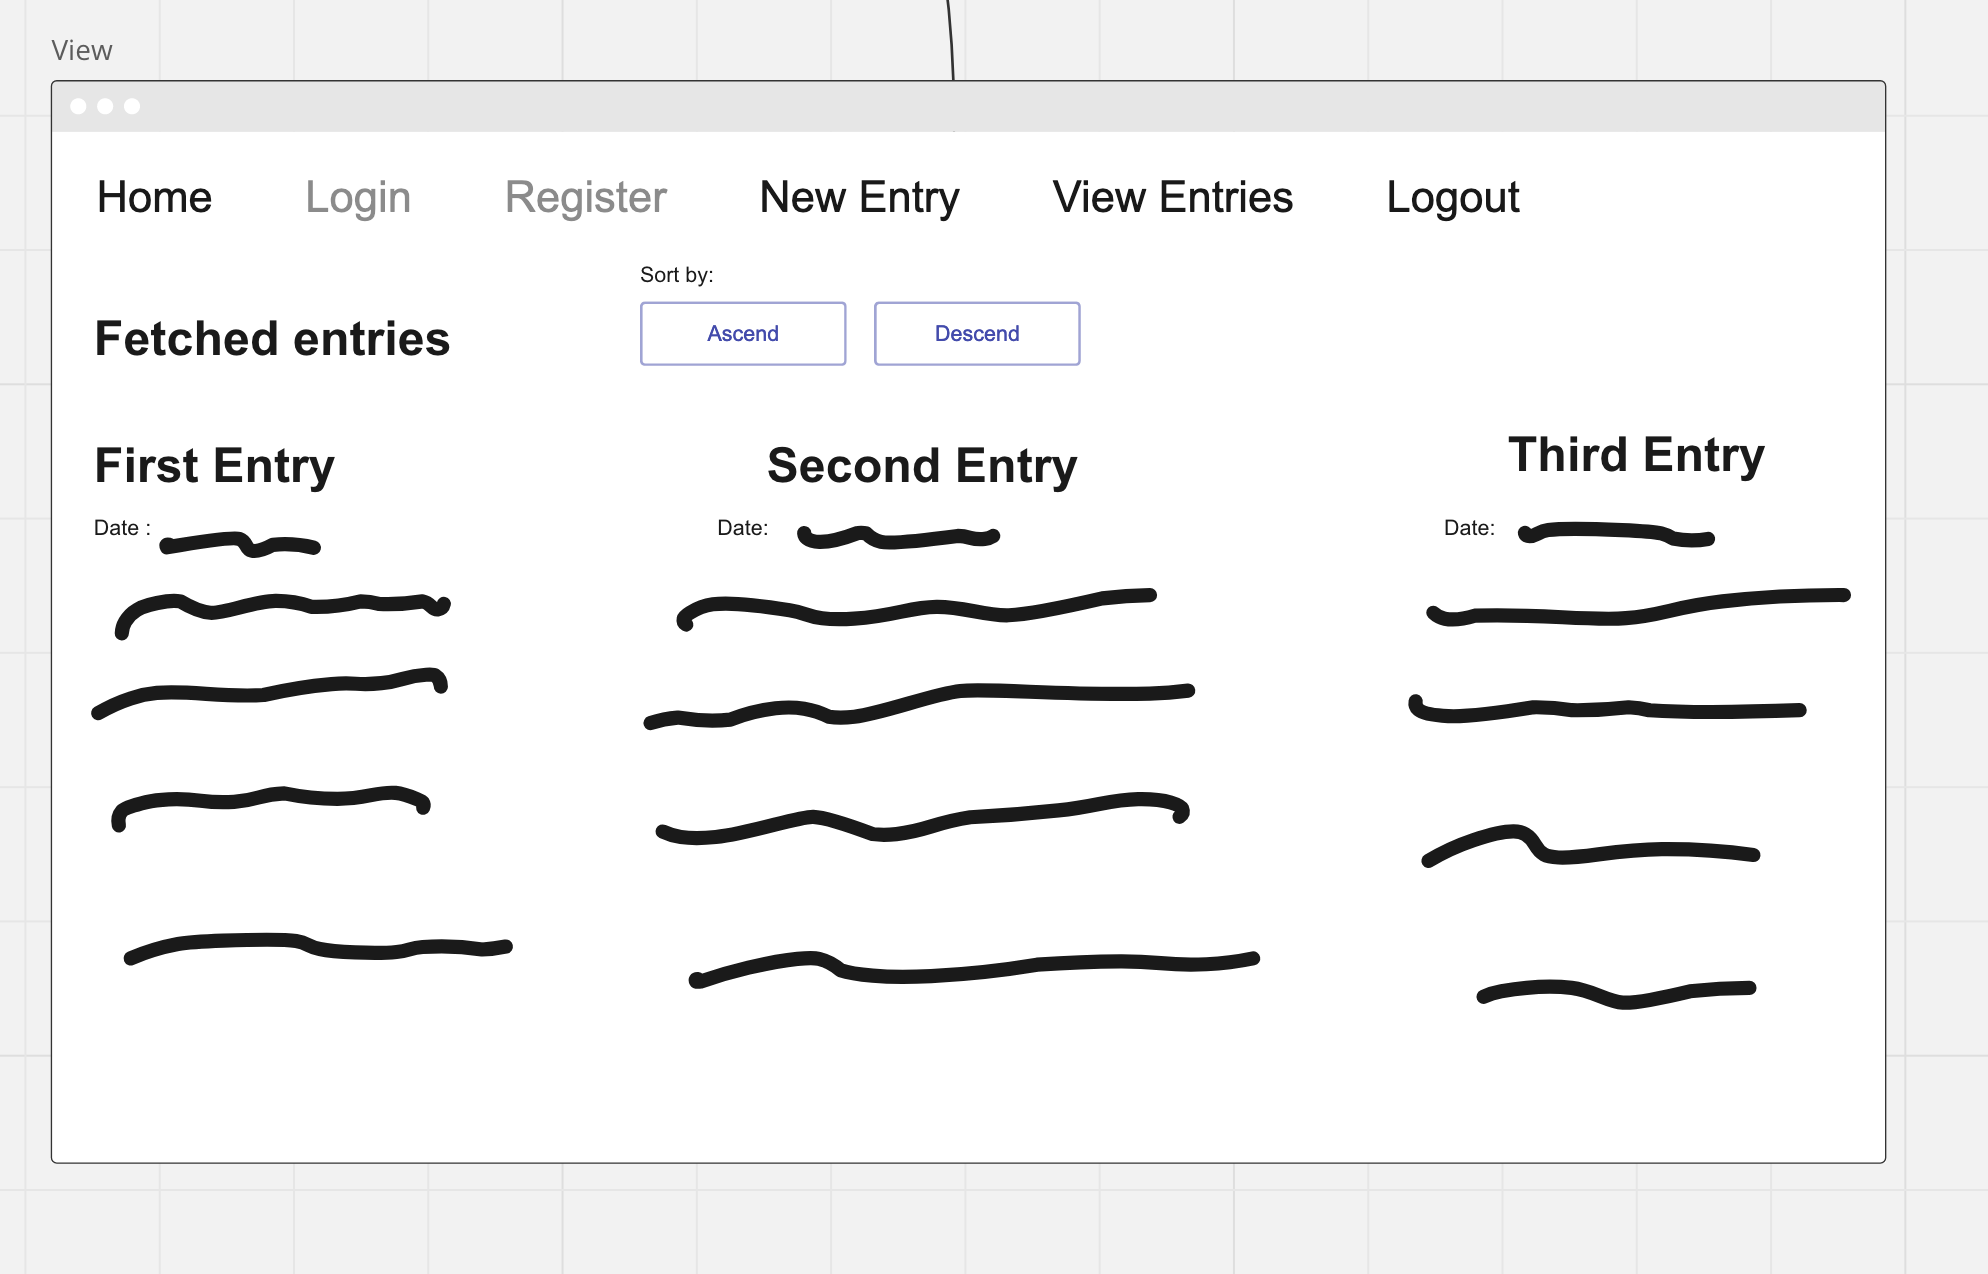
\includegraphics[width=0.8\textwidth]{Assets/view_page.png}
    \caption{View page is where the user can view all of their journal entries. It includes buttons to enable users to sort the entries.}
\end{figure}


\section{RESTful API Endpoints}
REST effectively allows my frontend application to directly interact with the server through HTTP requests. in this section I will document some of the endpoints I have created in my Django backend. One more thing to add is that I have used Django REST framework to create my API endpoints. This is a framework on top of Django specifically designed for creating RESTful APIs.

\subsection{Serialization and deserialization of data}
Serialization refers to the process of converting complex data type into a format that can easily be transmitted. For my case I need to break down the user object into a JSON format which can then be sent to and use in my frontend. Deserialization is the opposite process, where the JSON data is converted back into a complex data type. I would need to process the JSON data in the frontend, and the fact that I'm using javascript means that I can easily parse the JSON data, considering that JSON is a subset of JavaScript.

\subsection{login}
The login endpoint is used to authenticate the user. The user sends a POST request to the server with their email and password. The server then checks if the email and salted and hashed value of the password match with records in the database. If they do, the server generates a token and sends it back to the user. This token then can be used to authenticate future requests. For both login and register if successful serialized user data is sent back to the user along with the token.

\subsection{register}
Register is similar, but it is used to create a new user. The user sends a POST request with their email and password and other user information. The server first of perform sanity check on the format of the email via regex, then it checks if the email is already in use. If it is not, the server creates a new user with the email and password and sends back a token as well as other user details in the response.


\subsection{get entries}
This is the endpoint that retrieves all the entries of the user. The user sends a GET request, however the caveat is that the user must be authenticated and the generated token must be attached in teh header of the request. Because the user is validated, the server knows who this user is, and can then retrieve all the entries associated with this user through the foreign key relationship in the database. The server then sends back the entries in JSON format.

\subsection{create entry}
Create entry is used to create a new entry. The user sends a POST request with the title and content of the entry. For this method the user must also be authenticated. The server knows which user this is and through the one to one relationship between the user and the journal entry, the server can create a new entry and associate it with the user's journal. The server then sends back the status of the request. Otherwise it sends back an error message.

\subsection{get statistics}
This endpoint is used to obtain statistics about a user's journal. The server generate statistics based on the user's journal entries. 

\section{Interface Logic}
Here I have created flowcharts demonstrating how each of these web pages are suppose to function.

\subsection{Login and Register Page}
\begin{figure}[H]
    \begin{minipage}{0.48\textwidth}
        \centering
        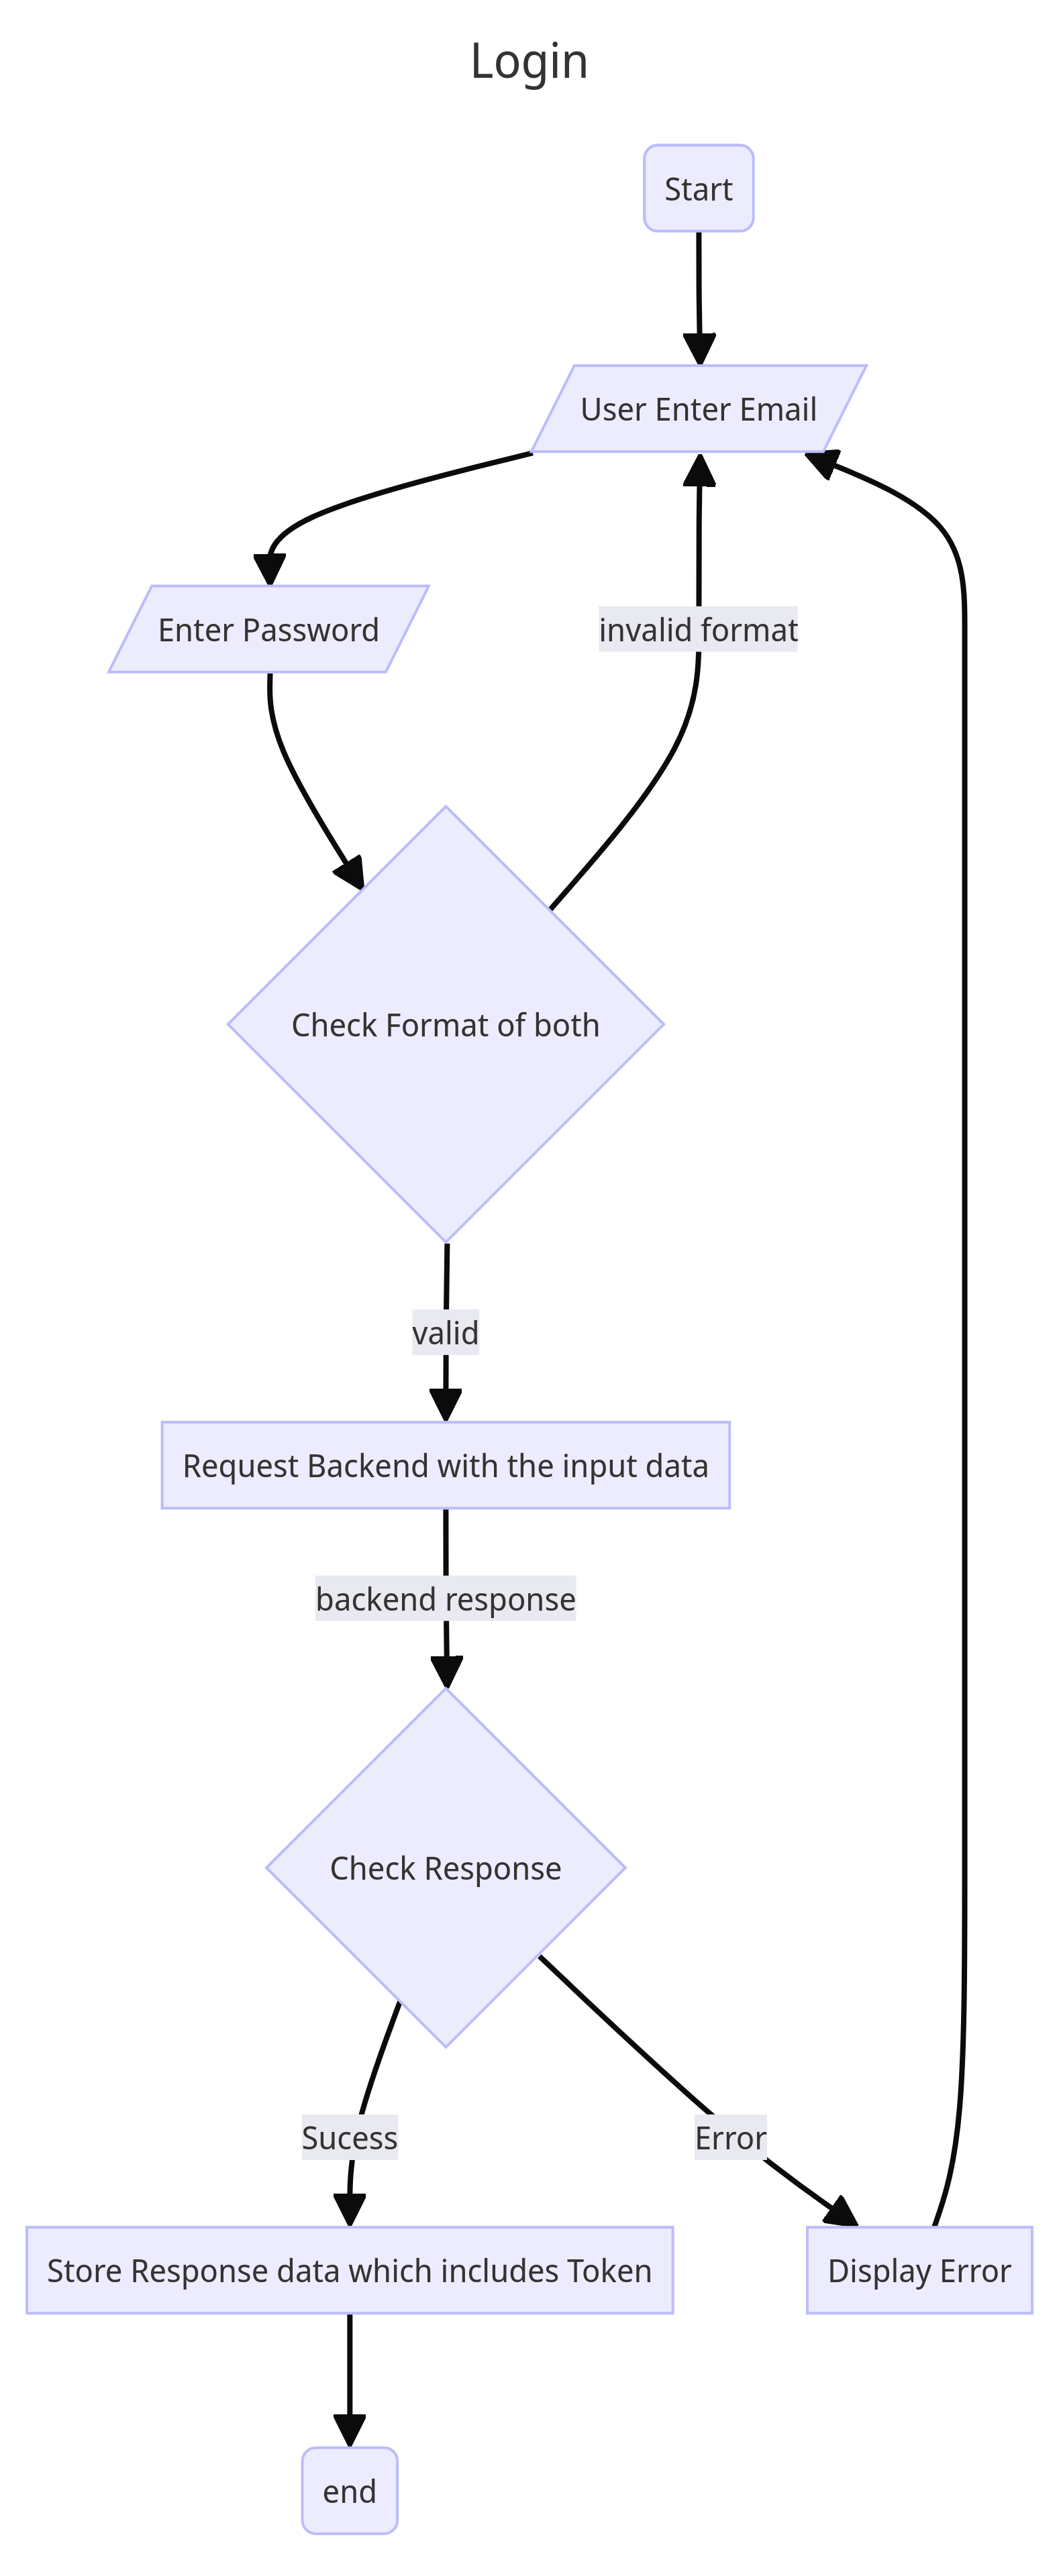
\includegraphics[width=\textwidth,height=\textheight,keepaspectratio]{Assets/loginPageFlow.png}
        \caption{Login Page}
    \end{minipage}\hfill
    \begin{minipage}{0.48\textwidth}
        \centering
        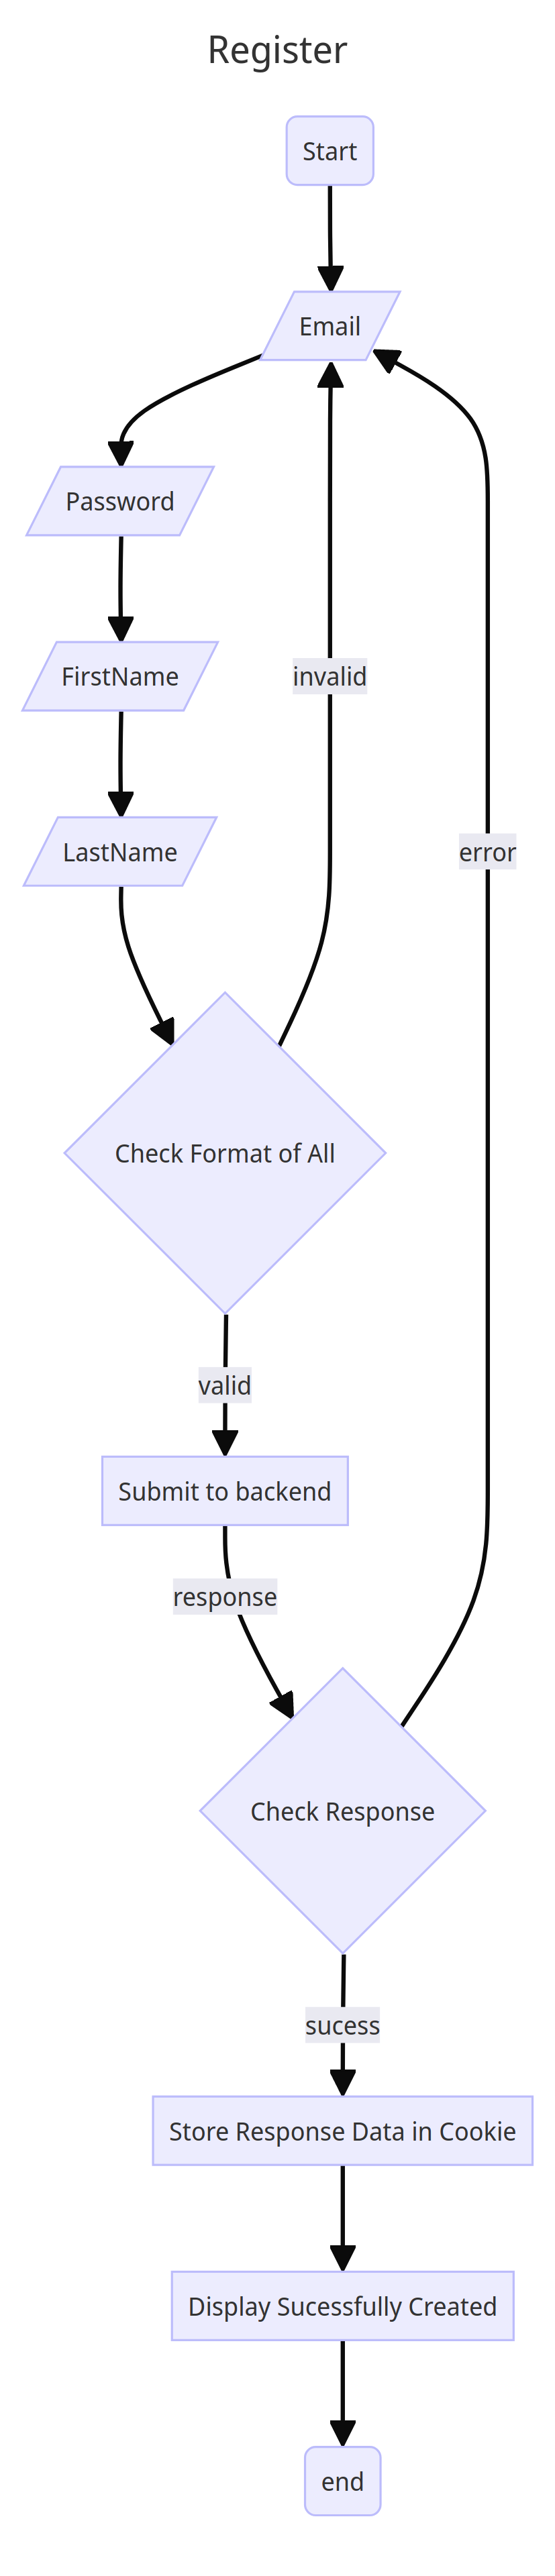
\includegraphics[width=\textwidth,height=0.8\textheight,keepaspectratio]{Assets/registerPageFlow.png}
        \caption{Register Page}
    \end{minipage}
\end{figure}

\subsection{Retrieve Entries Page}
\begin{figure}[H]
    \centering
    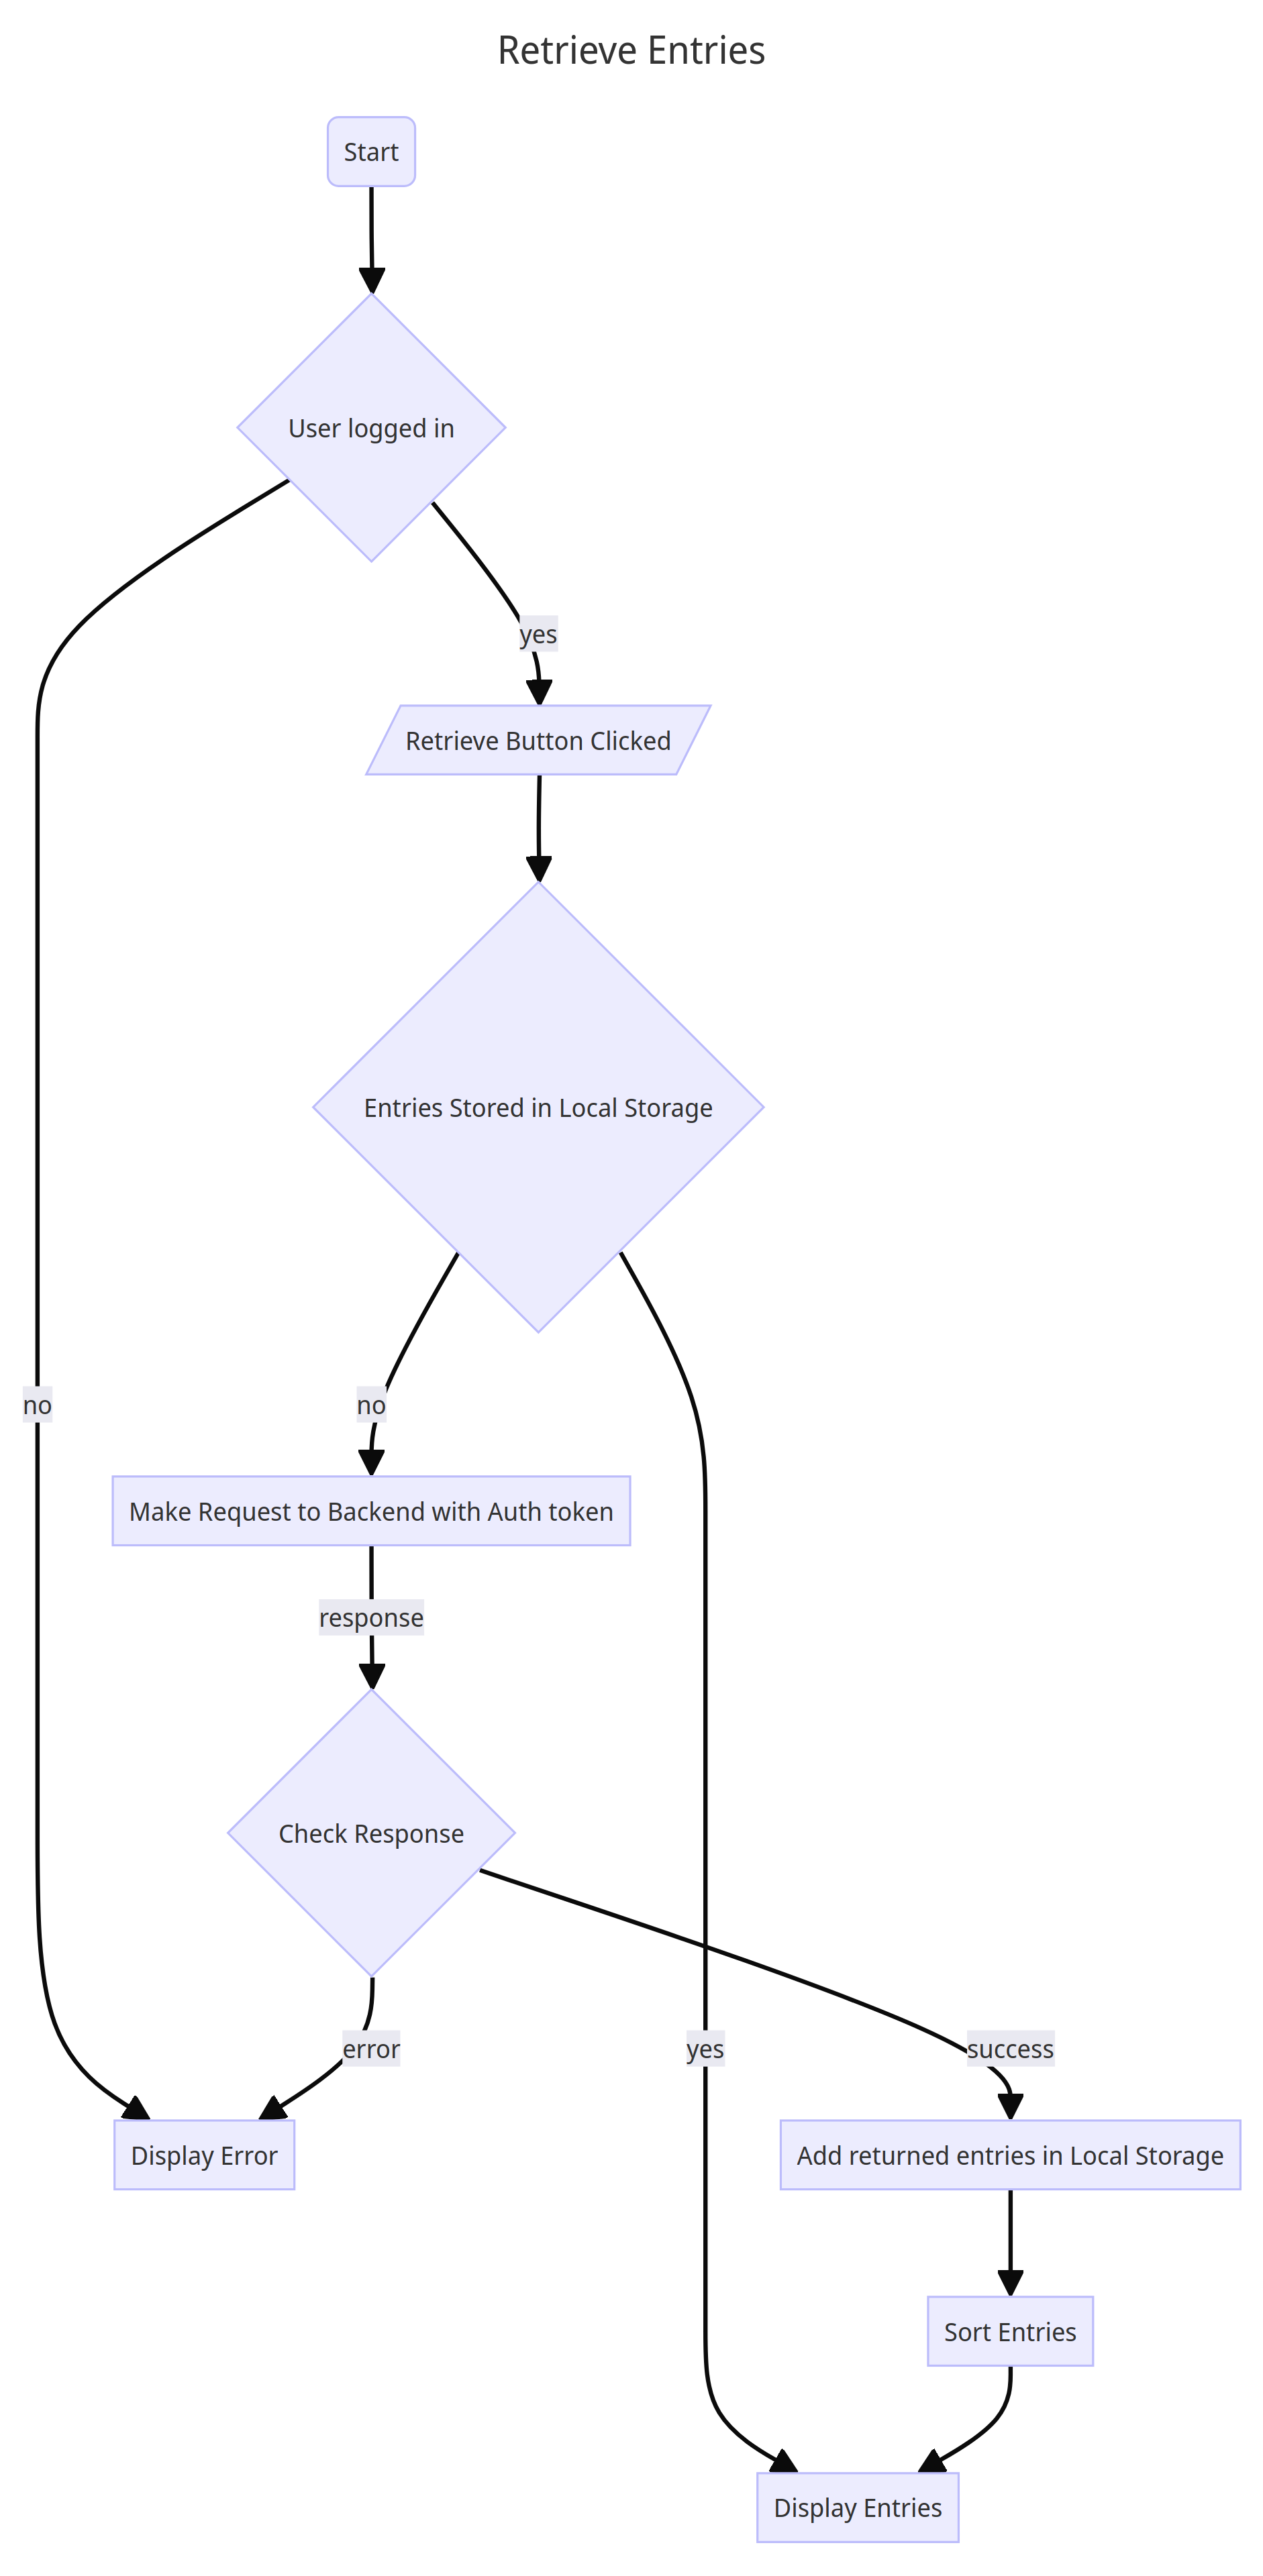
\includegraphics[width=0.6\textwidth]{Assets/retrievePageFlow.png}
    \caption{Retrieve Entries Page}
\end{figure}


\subsection{Other}
Create entries follow a similar design to login as it takes in user input and sends it to the server. The profile page is a page that displays the user's information, it reads of the data stored in my browser's storage then renders it. The home page is the first page the user sees when they visit the website. It includes buttons to navigate to other pages. 

\section{Generating User Statistics}
The statistics page renders the statistics generated by the server. The server use advance SQL queries to generate the statistics, and then sends it back to the user. Here I will be detailing the design of those queries.

\subsection{SQL Queries}
The exact implementation can be found in the Implementation section of the report. Here I will be detailing how the queries are structured and how they work.

\subsubsection{Most Active Month}
Here what happens is 


\section{Hardware \& Software Requirements}
Specify the hardware and software requirements for the project.

\begin{table}[H]
    \centering
    \begin{tabular}{|l|p{10cm}|}
    \hline
    \textbf{Requirement ID} & \textbf{Description} \\ \hline
    1 & Development Machine: Apple MacBook Pro 14-inch with M1 chip, 8 GB of RAM, and 256 GB SSD. This is more than sufficient for my development, React and Python are also well supported on Apple Silicone. \\ \hline
    2 & Server for Deployment: Initially it could be configured with 2 vCPUs, 4 GB RAM, and 50 GB SSD storage which should be enough for the backend, it should also be easily scalable. \\ \hline
    3 & End-User Devices: The app should be accessible on devices with internet connection and a web browser. This includes smartphone, laptop, even some smart IOT devices like your smart TV. \\ \hline
    \end{tabular}
    \caption{Hardware Requirements for Journal App}
    \end{table}

    
    \begin{table}[H]
        \centering
        \begin{tabular}{|l|p{10cm}|}
        \hline
        \textbf{Requirement ID} & \textbf{Description} \\ \hline
        1 & Development Environment: Visual Studio Code with the extensions for efficient coding. \\ \hline
        2 & Terminal: I use Alacritty as my terminal emulator, the default shell on my device is zsh. \\ \hline
        3 & Package Manager: Homebrew for macOS, very useful for installing new things for example postgres was installed through this. \\ \hline
        4 & Database: PostgreSQL, as well as pgAdmin 4 for database administration and interaction. \\ \hline
        5 & Backend Framework: Python, Django REST framework, which is also compatible with my database of choice. \\ \hline
        6 & Frontend Technologies: Typescript, React, Vite.js. \\ \hline
        7 & Version Control: Git for source code management, I use it to frequency commit my code, it is also synced with Github for backup. \\ \hline
        8 & Deployment: Many options are available if I were to host my application, notably ones commonly used include Google Cloud, AWS, there are also ones built for easy deployment ones such as Railway, Heroku and Netlify. \\ \hline  
        \end{tabular}
        \caption{Software Requirements for Journal App}
        \end{table}
        
